\documentclass[12pt,titlepage]{article}
\usepackage[spanish]{babel}
\usepackage[utf8]{inputenc}
\usepackage{amsmath}
\usepackage{amssymb}
\usepackage{graphicx}
\usepackage{caratulaMetNum}
\usepackage{float}
\usepackage{subfigure}
\usepackage{listings}
\lstset{language=C,basicstyle=\small\tt,keywordstyle=\bf,tabsize=3,breaklines=true,linewidth=16cm,postbreak={\mbox{$\rightsquigarrow$}},prebreak={\mbox{$\rightsquigarrow$}}}

 \usepackage{a4wide}
% \usepackage{amssymb}
% \usepackage{amsmath}
 \usepackage{enumerate}
% \usepackage[utf8]{inputenc}
% \usepackage[spanish]{babel}
% \parindent = 0 pt
 \parskip = 11 pt
% \usepackage[width=15.5cm, left=3cm, top=2.5cm, height= 24.5cm]{geometry}

\usepackage{color}
\usepackage{url}
\definecolor{lnk}{rgb}{0,0,0.4}
\usepackage[colorlinks=true,linkcolor=lnk,citecolor=blue,urlcolor=blue]{hyperref}

\newcommand{\func}[2]{\texttt{#1}(#2) :}
\newcommand{\tab}{\hspace*{2em}}
\newcommand{\FOR}{\textbf{for }}
\newcommand{\TO}{\textbf{ to }}
\newcommand{\IF}{\textbf{if }}
\newcommand{\WHILE}{\textbf{while }}
\newcommand{\THEN}{\textbf{then }}
\newcommand{\ELSE}{\textbf{else }}
\newcommand{\RET}{\textbf{return }}
\newcommand{\MOD}{\textbf{ \% }}
\newcommand{\OR}{\textbf{ or }}
\newcommand{\NOT}{\textbf{ not }}
\newcommand{\tOde}[1]{\tab \small{\mathcal{O}($#1$)}}
\newcommand{\Ode}[1]{\ensuremath{\small{\mathcal{O}\left(#1\right)}}}
\newcommand{\VSP}{\vspace*{3em}}
\newcommand{\Pa}{\vspace{5mm}}
\newenvironment{pseudo}{\noindent\begin{tabular}{ll}}{\end{tabular}\VSP}

\newenvironment{while}{\WHILE \\ \setlength{\leftmargin}{0em} }{}

\newcommand{\iif}{\Leftrightarrow}
\newcommand{\gra}[1]{\noindent\includegraphics[scale=.70]{#1}\\}
\newcommand{\gras}[2]{\noindent\includegraphics[scale=#2]{#1}\\}
\newcommand{\gram}[1]{\noindent\includegraphics[scale=.50]{#1}}
\newcommand{\dirmail}[1]{\normalsize{\texttt{#1}}}
\newenvironment{usection}[1]{\newpage\begin{section}*{#1}	\addcontentsline{toc}{section}{#1}}{\end{section}}
\newenvironment{usubsection}[1]{\begin{subsection}*{#1}	\addcontentsline{toc}{subsection}{#1}}{\end{subsection}}

\newcommand{\superref}[1]{\textsuperscript{\ref{#1}}}

%\title{{\sc\normalsize Métodos Numéricos}\\{\bf Trabajo Práctico Nº1}}
%\author{\begin{tabular}{lcr}Pablo Herrero & LU & \dirmail{pablodherrero@gmail.com}\\Thomas Fischer & 489/08 & \dirmail{tfischer@dc.uba.ar}\\Kevin Allekotte & 490/08 & \dirmail{kevinalle@gmail.com} \end{tabular}}
%\date{\VSP \normalsize{Abril 2010}}
\begin{document}

\materia{Métodos Numéricos}
\titulo{Trabajo Práctico Nº2}
\subtitulo{Chocan los Planetas...}
%\grupo{Grupo x}
\integrante{Pablo Herrero}{332/07}{pablodherrero@gmail.com}
\integrante{Thomas Fischer}{489/08}{tfischer@dc.uba.ar}
\integrante{Kevin Allekotte}{490/08}{kevinalle@gmail.com}

\abstracto{
	El siguiente trabajo se propone la comparación entre distintos
	métodos de simulación de sistemas gravitatorios
	de varios cuerpos usando resolución de sistemas lineales.
	El objetivo final es calcular las coordenadas para tirar
	un proyectil desde la órbita del planeta Neptuno para
	que el mismo impacte	en la Tierra.
}

\palabraClave{Simulación}
\palabraClave{Gravitación}
\palabraClave{Sistemas Lineales}
\palabraClave{Proyectil}

\begin{titlepage}
\maketitle
\end{titlepage}
\tableofcontents
\newpage

	\begin{usection}{Introducción teorica}

		En la mecánica classica o Newtoniana, el problema de lo $n$
		cuerpos es el problema de predecir el movimiento de cuerpos
		celestes en mutua interacción gravitatoria para cualquier
		instante en el futuro o deducir su movimiento en cualquier
		instante del pasado.

		La acción gravitatoria entre los cuerpos depende de las
		posiciones relativas entre ellos, por lo que las ecuaciones de
		interacción gravitatoria quedan definidas en términos de
		ecuaciones diferenciales.

		El problema que surge al plantear el problema con $3 \leq n$ es
		que las ecuaciones el sistema quedan definidas en función de
		demasiadas variables como para aplicar los métodos de integración
		conocidos hoy en día para resolver las ecuaciones.

		Luego tenemos que encontrar otra forma de calcular las
		variables. En nuestro caso elegimos el método de simulación,
		el cuál introduce errores analíticos por discretizar el tiempo y
		de redondeo por trabajar con la aritmética finita de la
		computadora, pero que tiene la ventaja que el sistema a resolver
		es lineal, para lo cuál conocemos un método.

		Para minimizar estos errores implementamos distintos métodos de
		cálculo numérico de aproximación que validamos con sistemas
		familiares como el sistema solar, del cual sabemos por ejemplo
		que las órbitas son elípticas y bastante estables. Si dibujamos
		las órbitas simuladas podemos ver si se comportan de manera
		similar a lo esperado. Además, tenemos datos que se supone son
		bastante precisos descargados de la web oficial de la NASA para
		comparar.

	\end{usection}

	\begin{usection}{Desarrollo}

		En primer lugar el desarrollo consistio en implementar módulos
		para las operaciones con y entre Matrices y Vectores que
		fuesen necesarios para resolver sistemas lineales. Esto
		implicaba también implementar el algoritmo de eliminación
		Gaussiana con pivoteo parcial para resolver el sistema lineal
		del segundo método de resolución. Los módulos fueron
		implementados en el lenguaje \texttt{C++} para garantizar una
		buena performance.
		
		Escribimos el módulo \texttt{Matriz.h} que implementa una matriz
		con las operaciones:
		
		\begin{tabular}{rl}
			\texttt{T} & Transpuesta\\
			\texttt{resolver} & Solución al sistema $Mx=b$\\
			\texttt{triangular} & Triangula la matriz con el método de eliminación gausseana con pivoteo simple\\
			\multicolumn{2}{l}{
				\texttt{Suma, Resta, Multiplicación, Multiplicación por escalar}
			}
		\end{tabular}
		
		Elegimos implementar la triangulación con el método gausseano
		de pivoteo simple porque es una de las formas más simples para
		resolver un sistema de ecuaciones lineal.
		
		Además escribimos la clase \texttt{Vector3} que implementa un vector
		en $\mathbb{R}^3$ con las operaciones básicas como \texttt{Suma, Resta
		Producto Escalar, Producto Vectorial, Normalizar}, etc.

		Luego procedimos a implementar un entorno de simulación
		(\texttt{C++}) y un pequeño script para plotear y poder
		visualizar los resultados (\texttt{Python}). 

		Con todo el backend funcionando, procedimos a implementar
		gradualmente los distintos algoritmos de solución de sistemas
		lineales, intercalando la producción de cada uno, con fases de
		validación que consistían en simular los sistemas propuestos
		en el enunciado, y cuyos resultados se pueden observar en la
		sección \textbf{resultados}.
		
		Para validar los métodos utilizados en la simulación corrimos pruebas
		que consistían en casos simples como por ejemplo Sol-Tierra-Luna, o el
		sistema solar y observamos si las trayectorias de los cuerpos se comportaban
		como esperadas. Por ejemplo comprobamos si la órbita de la tierra alrededor del
		sol era aproximadamente circular y si recorría una vuelta entera en 365 días.
		Ademas vimos si la trayectoria de la luna parecía acompañar a la tierra.
		Observamos que con un $dt$ de una hora los planetas se comportaban suficientemente
		parecido a lo que esperábamos.

		Validados los métodos de simulación, tuvimos que idear un
		algoritmo para calcular el vector de velocidad inicial de
		nuestro proyectil dirigido a la tierra, de tal manera que le pegase.
		La idea fue hacer una especie de búsqueda local, ya que
		suponíamos que de no colisionar con otro planeta en la
		trayectoria hasta la tierra, si pasabamos con una trayectoría
		mas cerca de la tierra que con otra, podíamos reducir la
		búsqueda de la solución a un espacio localizado cerca de la
		primera. Con un espacio o una trayectoria nos referimos a una
		velocidad inicial, la que en nuestro código esta determinada por
		dos ángulos de disparo. Uno alrededor el eje $\hat{z}$, sobre el
		plano $\hat{x}\hat{y}$ ($\phi$) y otro alrededor del eje $\hat{y}$, sobre
		el plano $\hat{x}\hat{z}$ ($\theta$).
		
		Dadas las condiciones iniciales de un sistema (posiciones y velocidades de todos los cuerpos), podemos simular este sistema con alguno de los métodos y calcular las posiciones para algun tiempo en el futuro.
		Nuestro objetivo es encontrar la velocidad inicial de nuestro proyectil para que esté a menos de $10^{-4}$ AU de la tierra en algun instante futuro.
		Definimos entonces una función (\texttt{mindist}) que dadas las condiciones iniciales, un cuerpo \texttt{proyectil} y un cuerpo \texttt{target}, nos devuelva la distancia mínima a la que se encontrarán estos cuerpos en algun futuro acotado.
		Nos restringimos a los casos en los que la distancia es monótonamente decreciente, y consideramos sólo los tiempos para los cuales los cuerpos se acercan. (Esto es una desicion de implementación, ya que no estaríamos encontrando las soluciones en las que el proyectil se aleja y luego se vuelve a acercar).
		
		Como posición de lanzamiento elegimos un punto aproximadamente sobre la
		órbita de neptuno, esto es, a unos 30AU del sol, sobre el plano $xy$.
		Por ejemplo, los lanzamientos de prueba tenían como posición inicial el punto $(30,0,0)$.
		
		Tenemos entonces que minimizar esta función (o encontrar un valor para el cual sea menor que $10^{-4}$).
		Para esto elegimos una velocidad inicial a mano (aproximadamente hacia el cuerpo \texttt{target}) y corremos un algoritmo que va ajustando la velocidad para minimizar la función \texttt{mindist}. [Más detalles en \textbf{Discusión}]

		\begin{figure}[H]
			\centering
			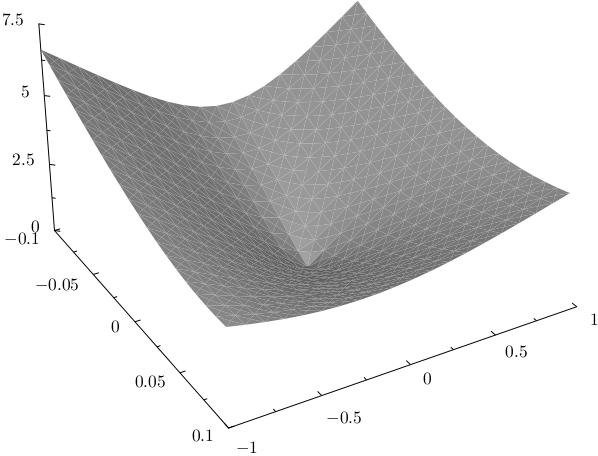
\includegraphics[scale=0.6]{mindist3.png}
			\caption{Esta es la forma de la función \texttt{mindist} para ciertas condiciones iniciales, donde el dominio es $\phi\times\theta$ (la velocidad inicial del proyectil) y la imagen es la distancia mínima.}
			\label{fig:mindist}
		\end{figure}	

	\end{usection}
	\begin{usection}{Resultados}
	\label{sec:res}
%		\begin{figure}
	\centering
	\subfigure[$\Delta t$ = 1 día]{
	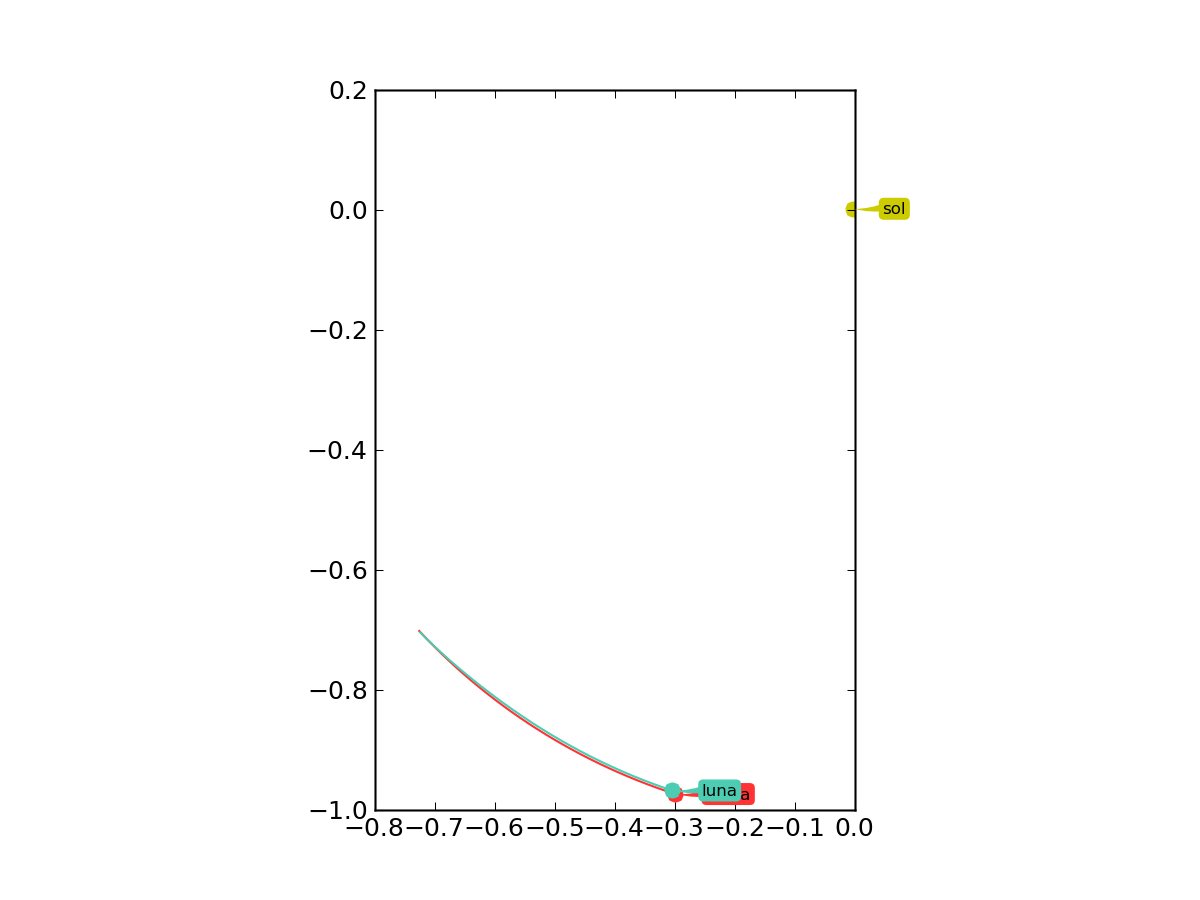
\includegraphics[scale=0.38]{img/ej1/metodo1/validacion_30_1.png}
	\label{fig:ej1_m1_30_1}
	}
	\subfigure[$\Delta t$ = 6 horas]{
	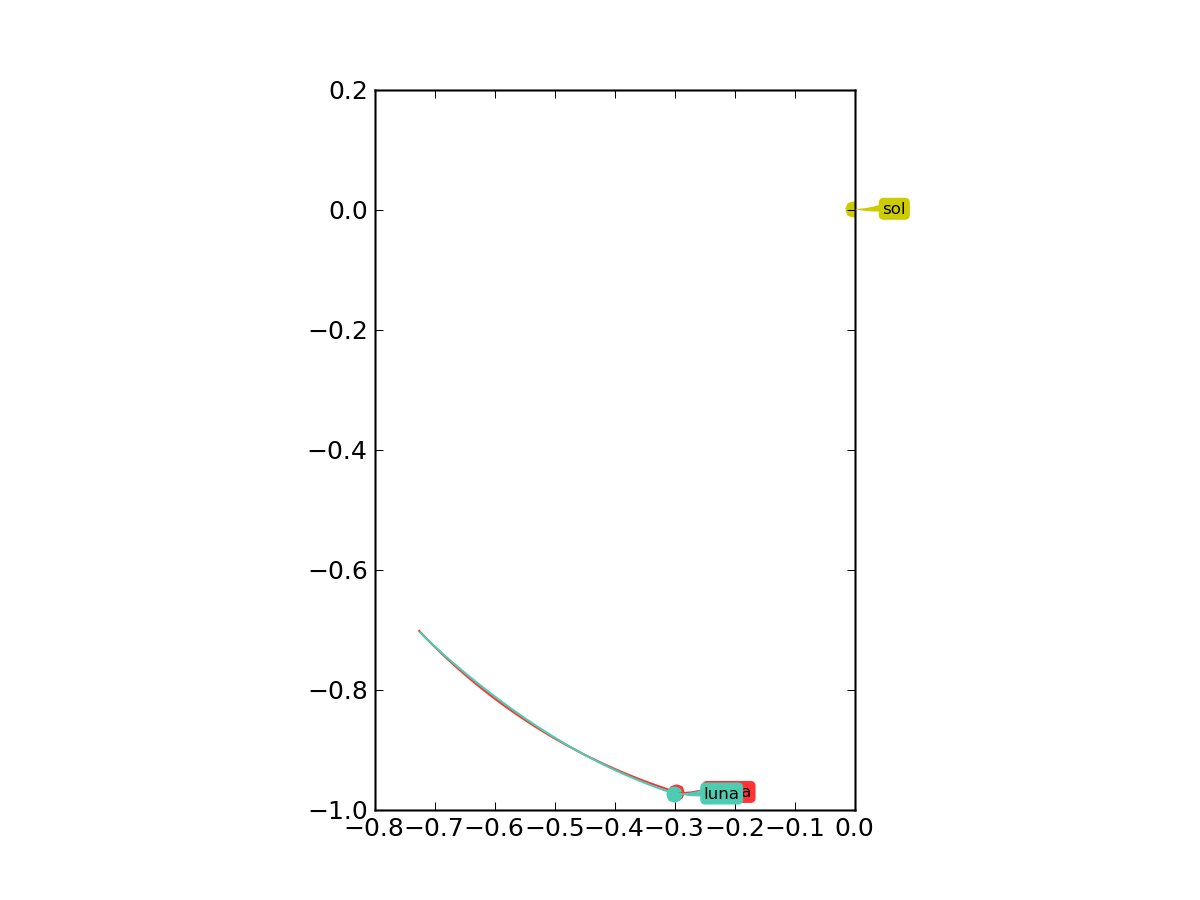
\includegraphics[scale=0.38]{img/ej1/metodo1/validacion_30_4.png}
	\label{fig:ej1_m1_30_4}
	}
	\\
	\subfigure[$\Delta t$ = 2 horas]{
	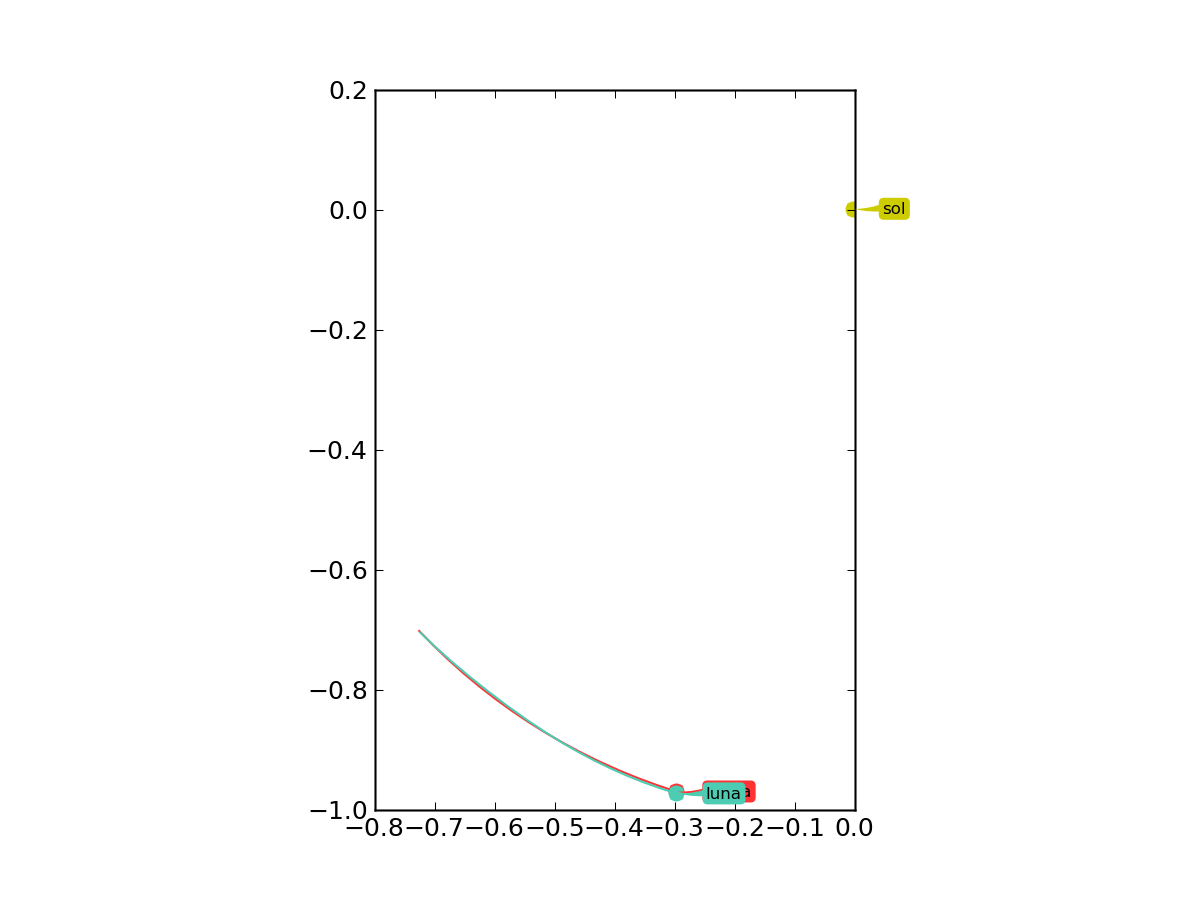
\includegraphics[scale=0.38]{img/ej1/metodo1/validacion_30_12.png}
	\label{fig:ej1_m1_30_12}
	}
	\subfigure[$\Delta t$ = 1 hora]{
	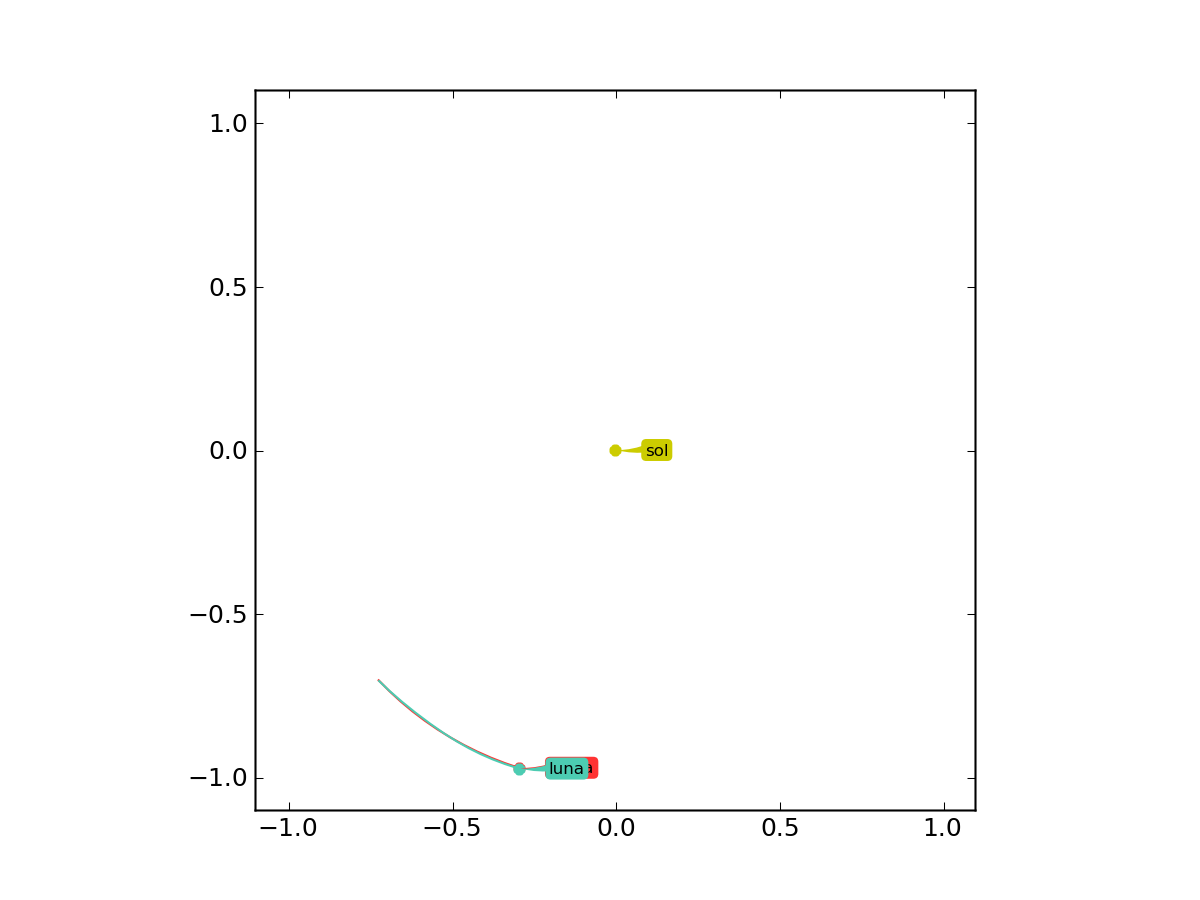
\includegraphics[scale=0.38]{img/ej1/metodo1/validacion_30_24.png}
	\label{fig:ej1_m1_30_24}
	}
	\caption{
		Simulación de validación del sistema sol$-$tierra$-$luna para un período de 30 días y distintos $\Delta t$
		con el método 1.
		Observamos que el error no parece ser tan grande a simple vista para este período.
	}
	\label{ fig:res_ej1_m1_30 }
\end{figure}
\begin{figure}
	\centering
	\subfigure[$\Delta t$ = 1 día]{
	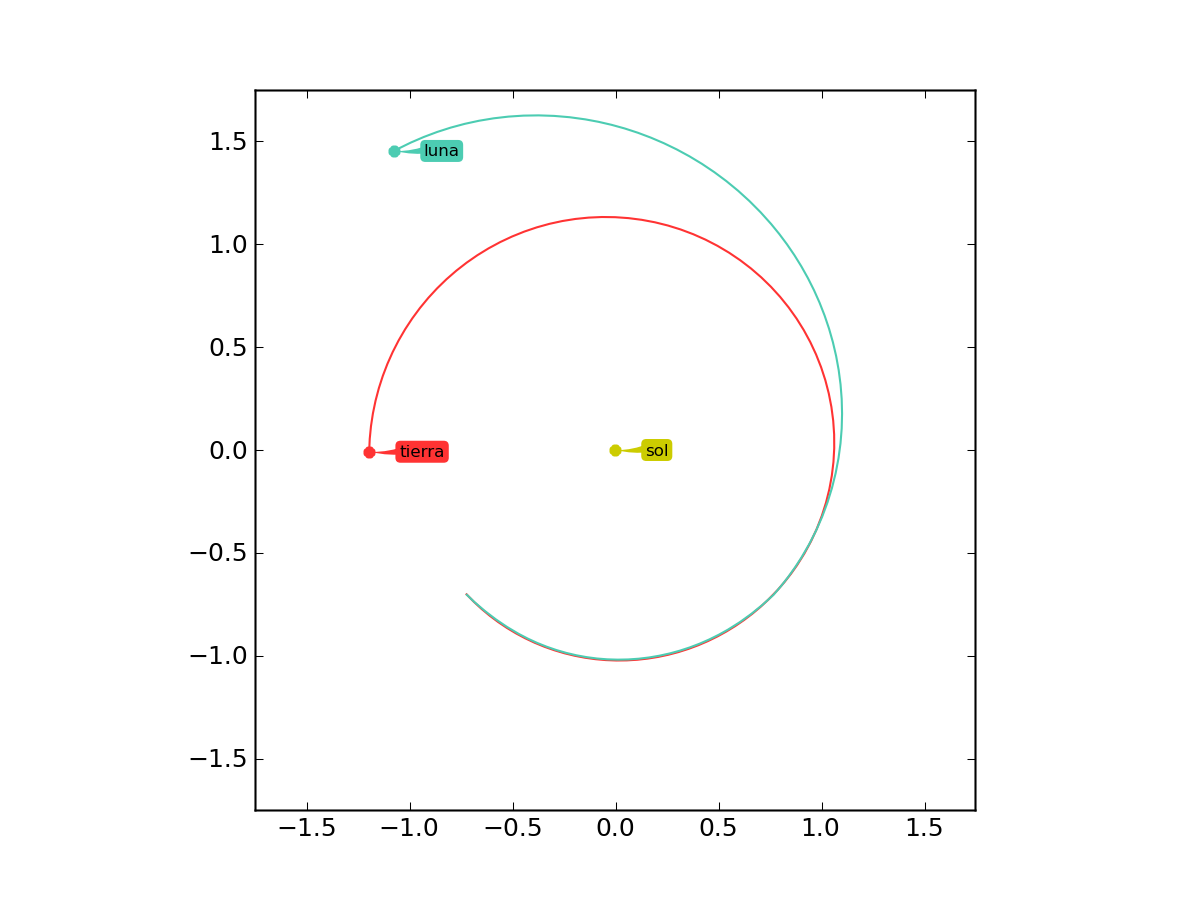
\includegraphics[scale=0.38]{img/ej1/metodo1/validacion_365_1.png}
	\label{fig:ej1_m1_365_1}
	}
	\subfigure[$\Delta t$ = 6 horas]{
	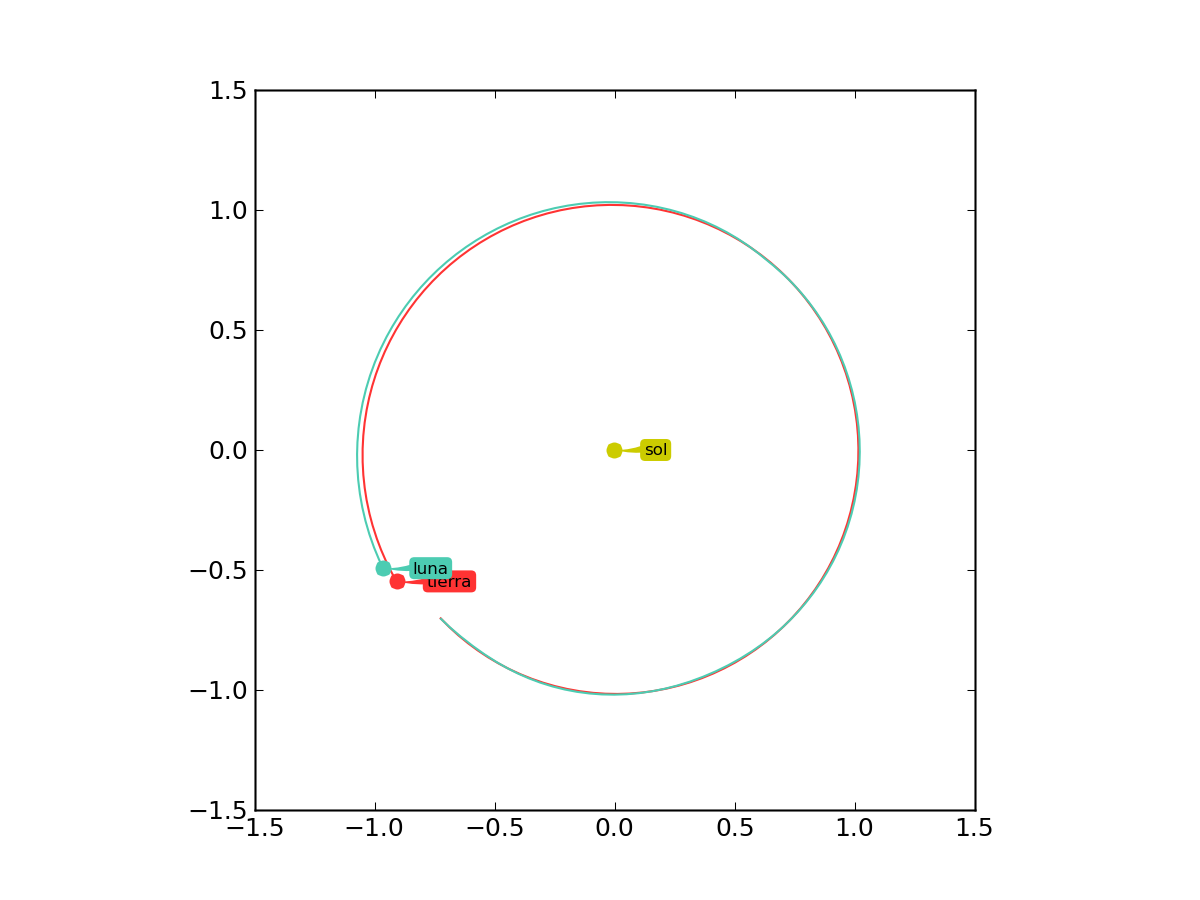
\includegraphics[scale=0.38]{img/ej1/metodo1/validacion_365_4.png}
	\label{fig:ej1_m1_365_4}
	}
	\\
	\subfigure[$\Delta t$ = 2 horas]{
	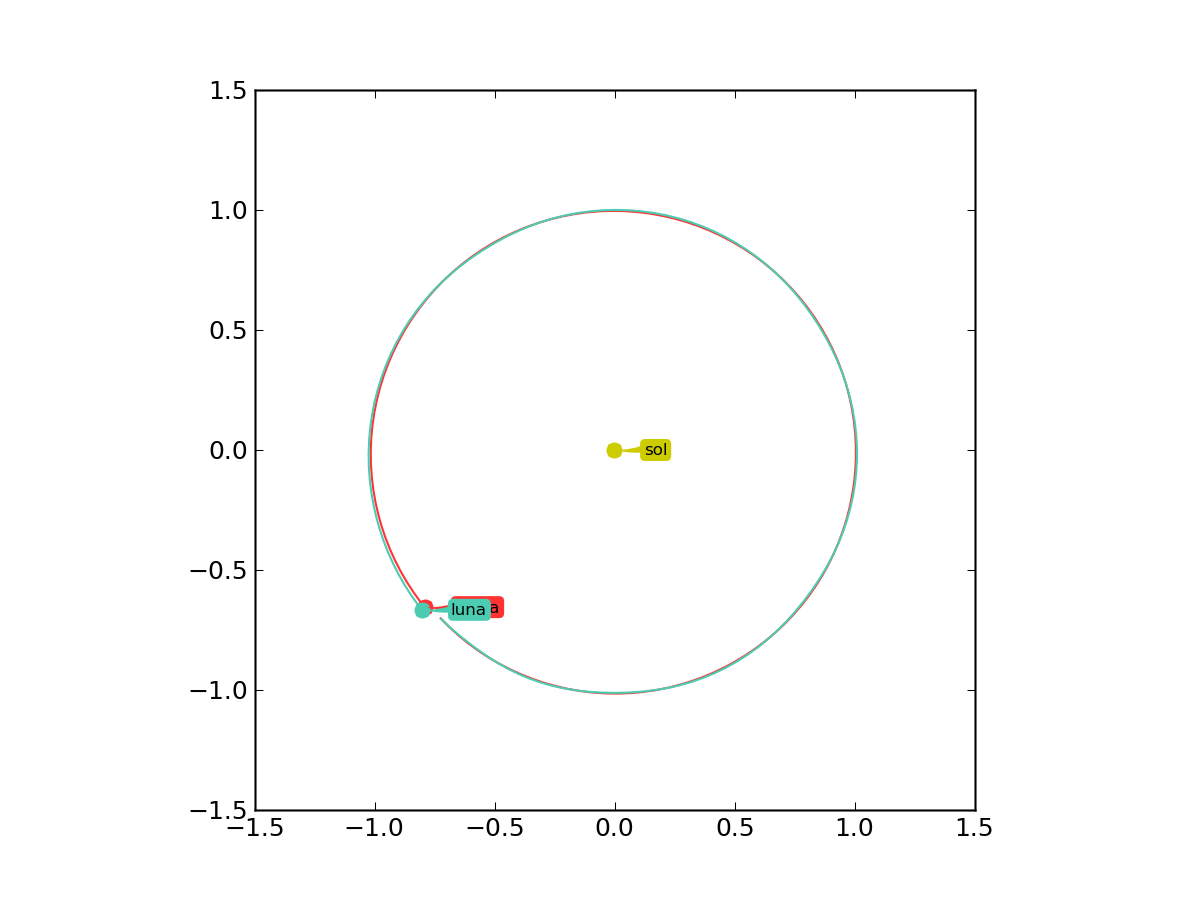
\includegraphics[scale=0.38]{img/ej1/metodo1/validacion_365_12.png}
	\label{fig:ej1_m1_365_12}
	}
	\subfigure[$\Delta t$ = 1 hora]{
	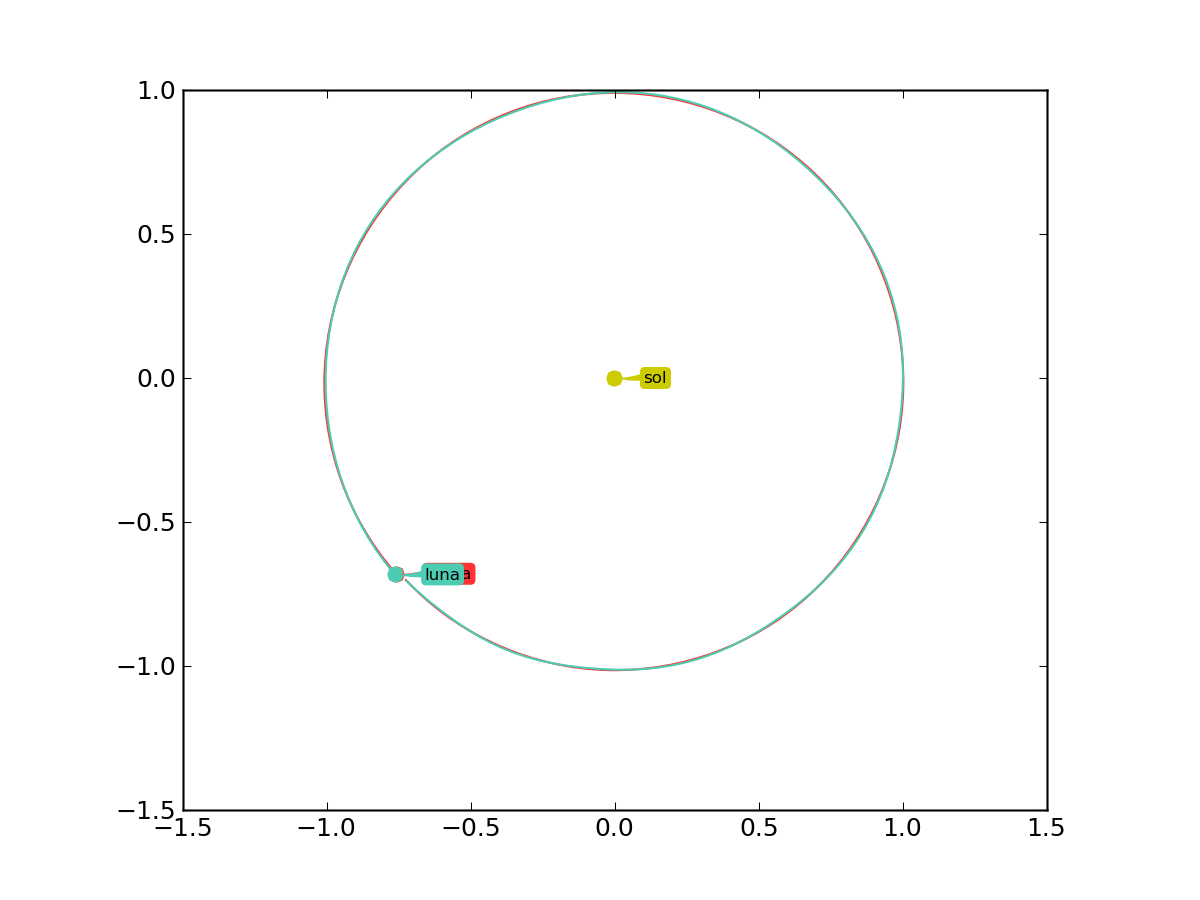
\includegraphics[scale=0.38]{img/ej1/metodo1/validacion_365_24.png}
	\label{fig:ej1_m1_365_24}
	}
	\caption{
		Simulación de validación del sistema sol$-$tierra$-$luna para un período de 1 año y distintos $\Delta t$
		con el método 1.
		Para esta cantidad de tiempo, la simulación con un $\Delta t$ de un día ya merece ser descartada.
		Las otras todavía parecen comportarse razonablemente
	}
	\label{ fig:res_ej1_m1_365 }
\end{figure}
\begin{figure}
	\centering
	\subfigure[$\Delta t$ = 1 día]{
	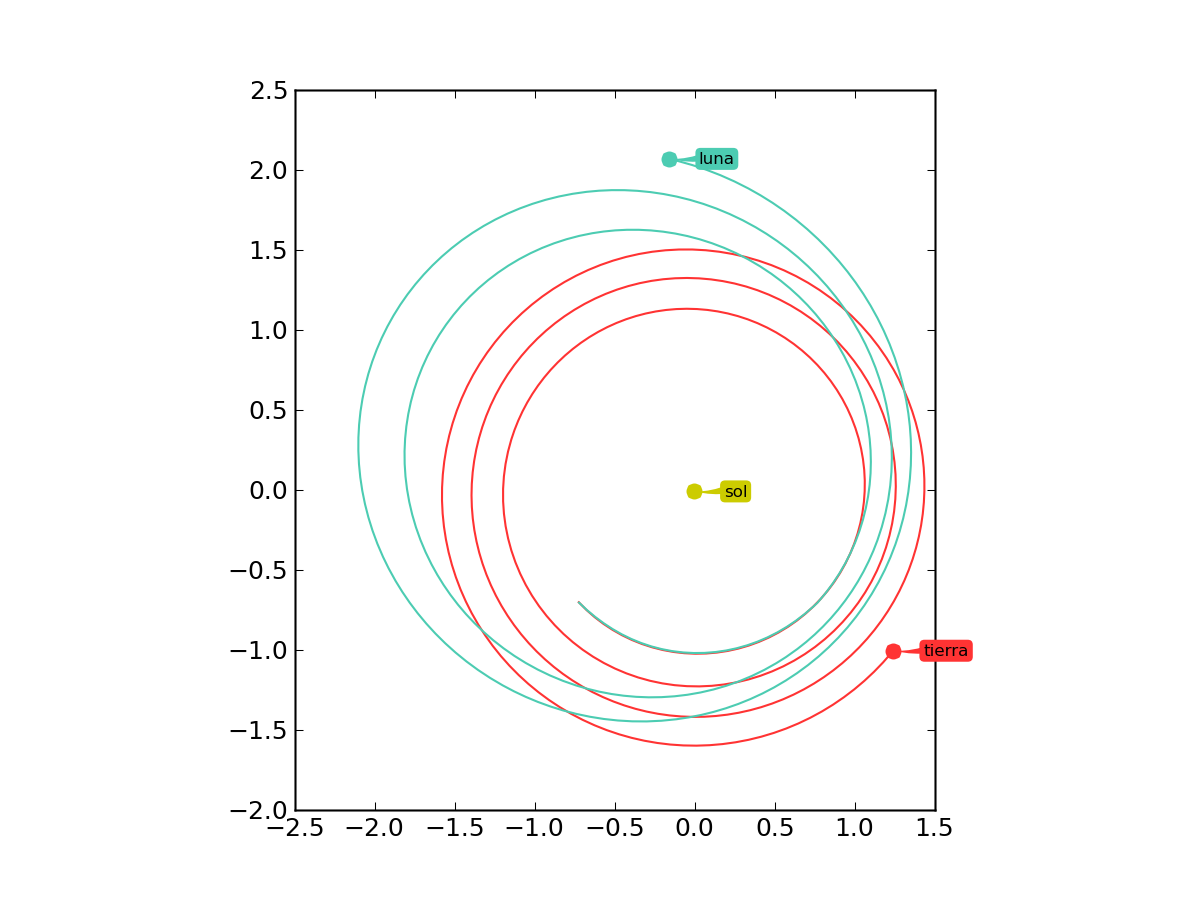
\includegraphics[scale=0.38]{img/ej1/metodo1/validacion_1825_1.png}
	\label{fig:ej1_m1_1825_1}
	}
	\subfigure[$\Delta t$ = 6 horas]{
	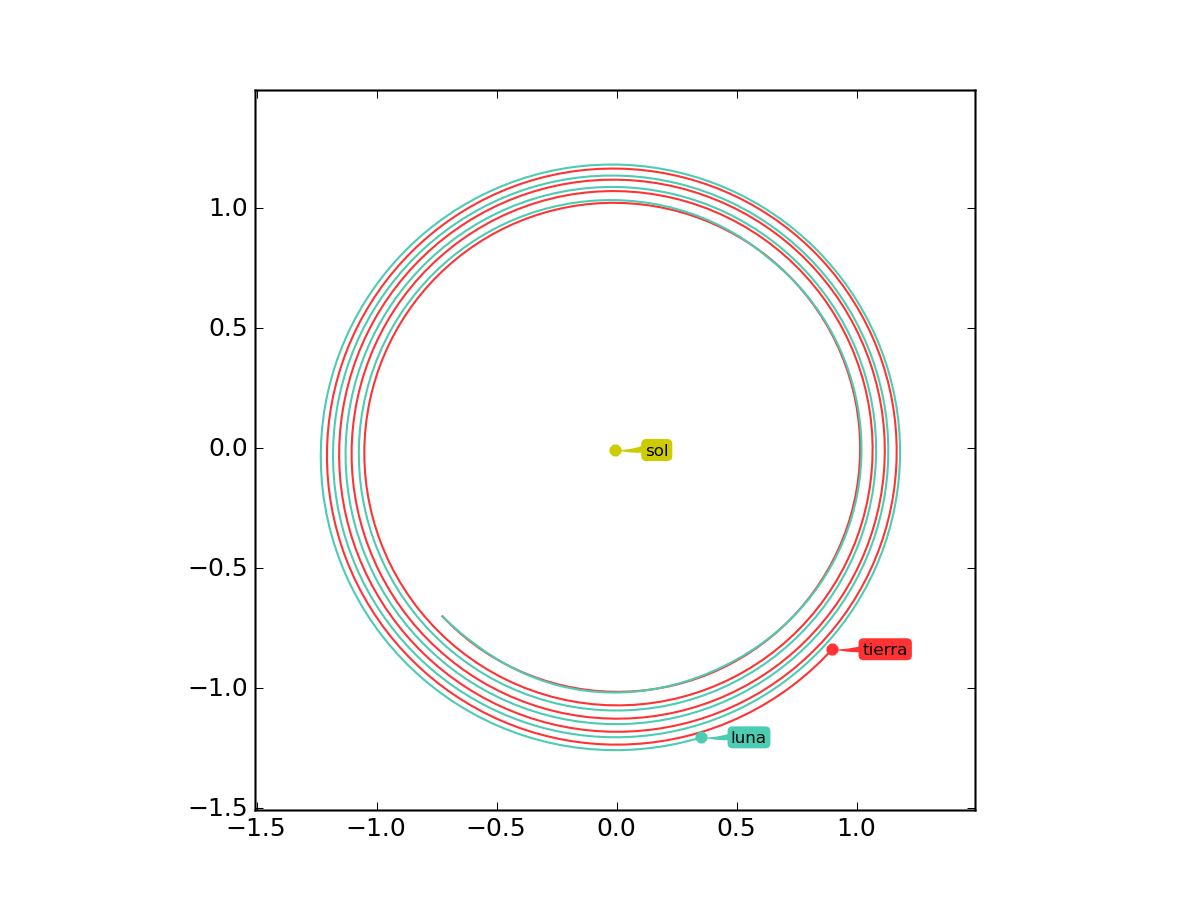
\includegraphics[scale=0.38]{img/ej1/metodo1/validacion_1825_4.png}
	\label{fig:ej1_m1_1825_4}
	}
	\\
	\subfigure[$\Delta t$ = 2 horas]{
	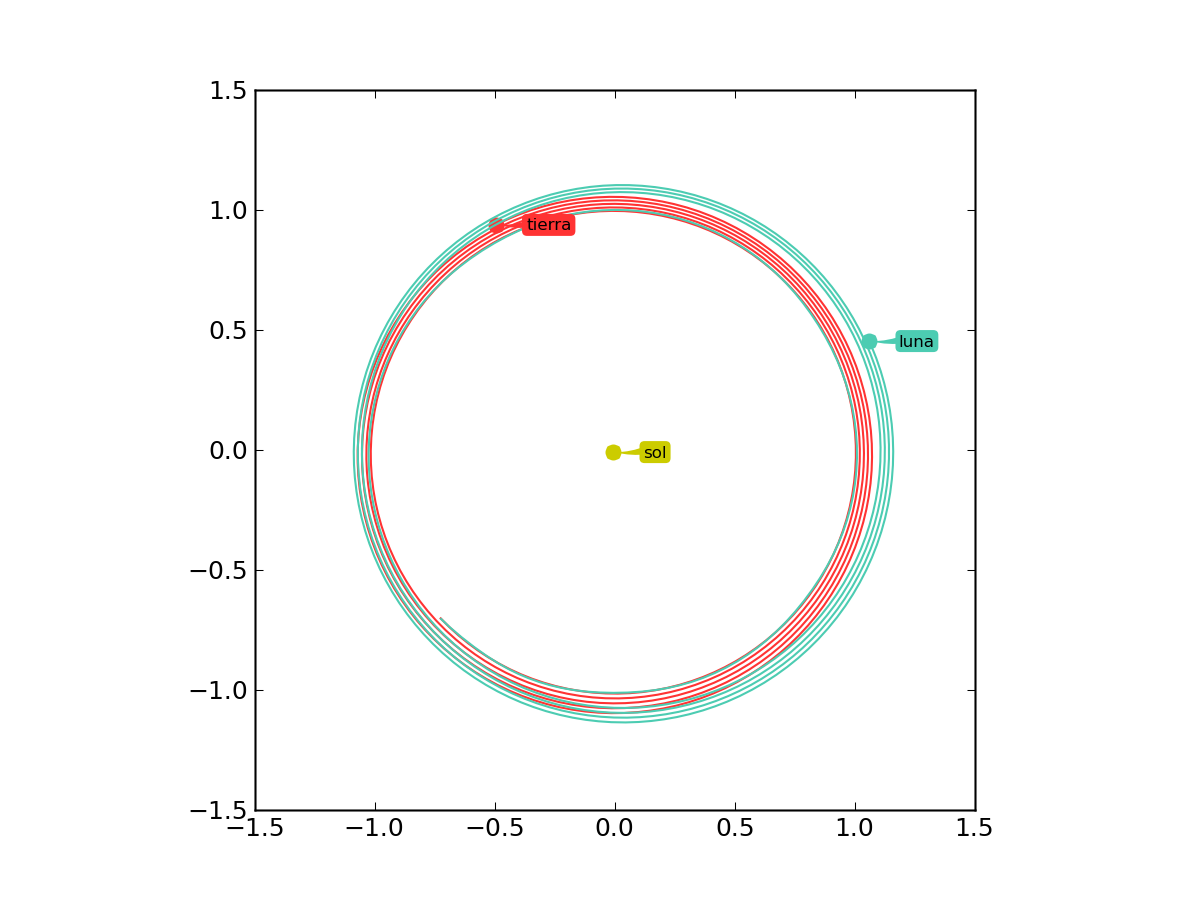
\includegraphics[scale=0.38]{img/ej1/metodo1/validacion_1825_12.png}
	\label{fig:ej1_m1_1825_12}
	}
	\subfigure[$\Delta t$ = 1 hora]{
	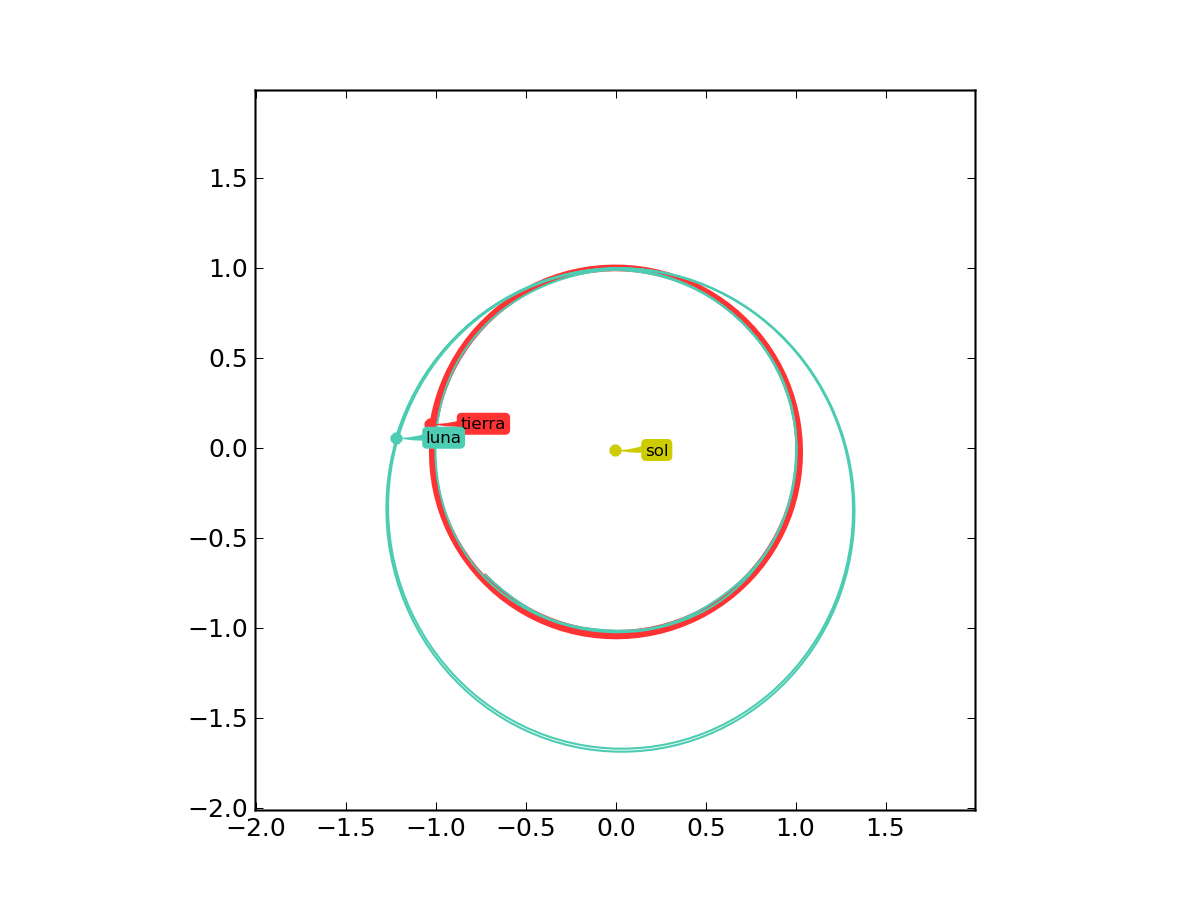
\includegraphics[scale=0.38]{img/ej1/metodo1/validacion_1825_24.png}
	\label{fig:ej1_m1_1825_24}
	}
	\caption{
		Simulación de validación del sistema sol$-$tierra$-$luna para un período de 5 años y distintos $\Delta t$
		con el método 1.
		Para esta cantidad de tiempo de simulación, las órbitas de los planetas ya comienzan a mostrar un movimiento espiral en vez de elíptico más de una vuelta.
		El mejor método parece ser el de $\Delta t$ de 2 horas, ya que para el de 1 hora la luna comienza a comportarse de una manera un poco mas extraña,
		comportamiento que atribuímos a errores de redondeo por tratar con numeros muy chicos o muy grandes al multiplicar o dividir respectivamente por un $\Delta t$ muy chico.
	}
	\label{ fig:res_ej1_m1_1825 }
\end{figure}

%		\begin{figure}
	\centering
	\subfigure[$\delta t$ = 1 día]{
	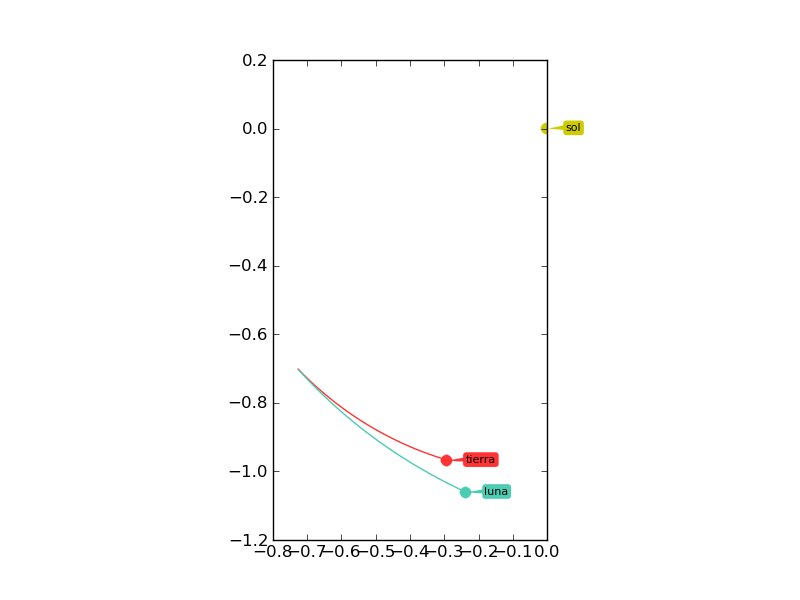
\includegraphics[scale=0.38]{img/ej1/metodo2/validacion_30_1.png}
	\label{fig:ej1_m2_30_1}
	}
	\subfigure[$\delta t$ = 6 horas]{
	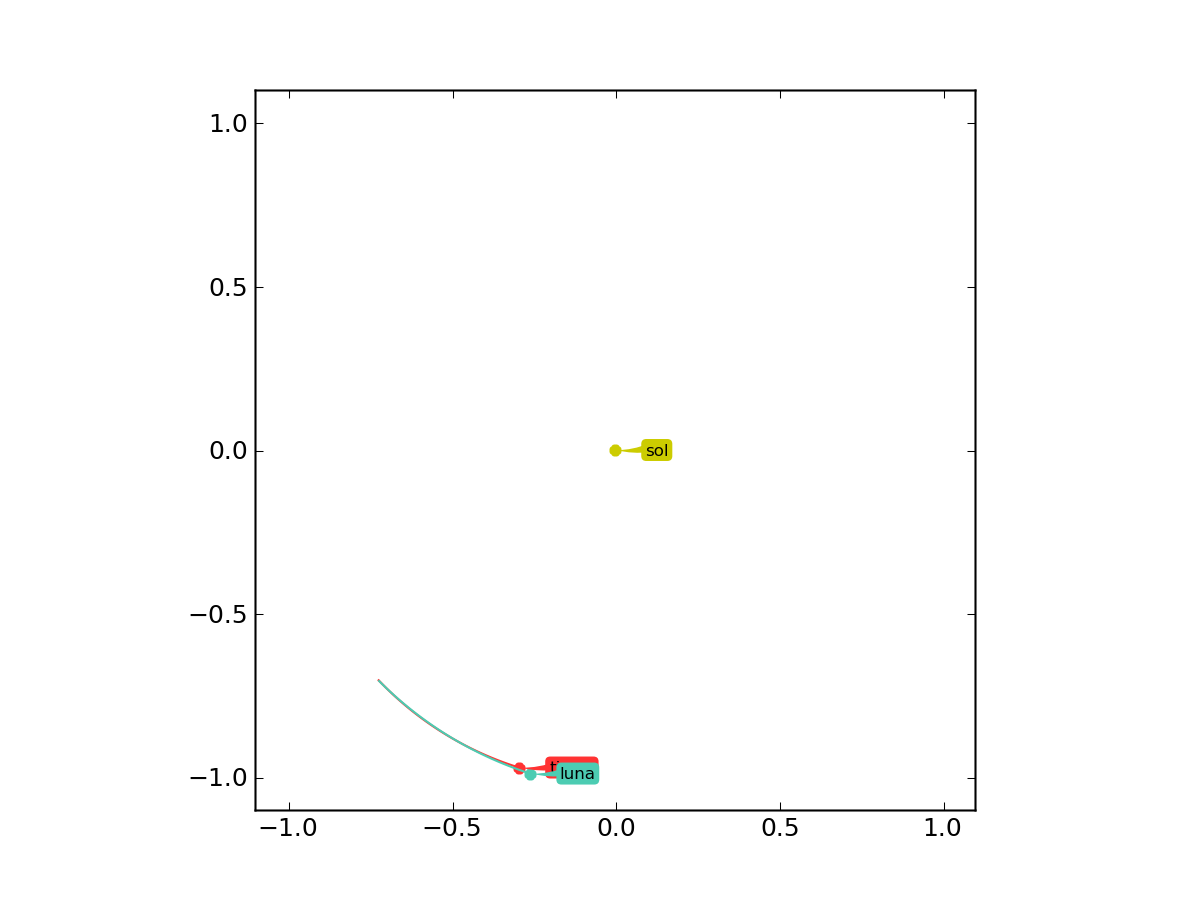
\includegraphics[scale=0.38]{img/ej1/metodo2/validacion_30_4.png}
	\label{fig:ej1_m2_30_4}
	}
	\\
	\subfigure[$\delta t$ = 2 horas]{
	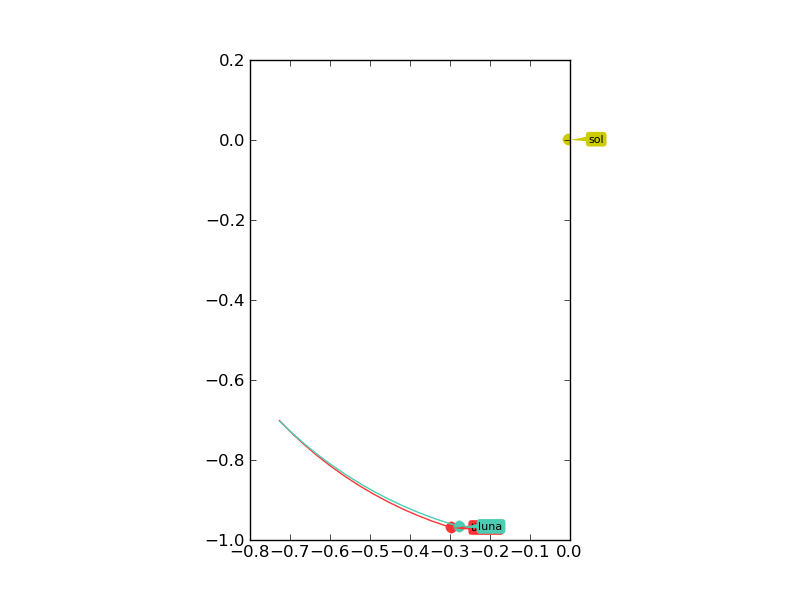
\includegraphics[scale=0.38]{img/ej1/metodo2/validacion_30_12.png}
	\label{fig:ej1_m2_30_12}
	}
	\subfigure[$\delta t$ = 1 hora]{
	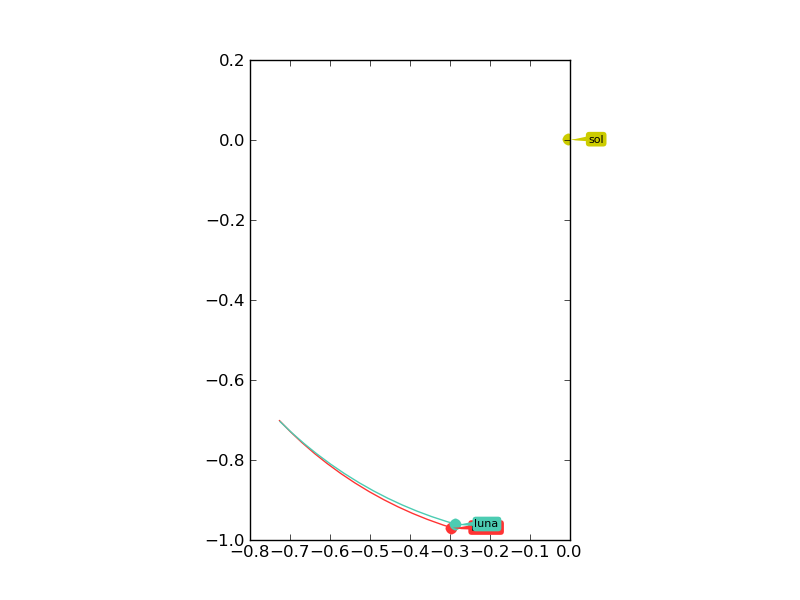
\includegraphics[scale=0.38]{img/ej1/metodo2/validacion_30_24.png}
	\label{fig:ej1_m2_30_24}
	}
	\caption{
		Simulación de validación del sistema sol$-$tierra$-$luna para un período de 30 días y distintos $\delta t$
		con el método 2.
	}
	\label{ fig:res_ej1_m2_30 }
\end{figure}
\begin{figure}
	\centering
	\subfigure[$\delta t$ = 1 día]{
	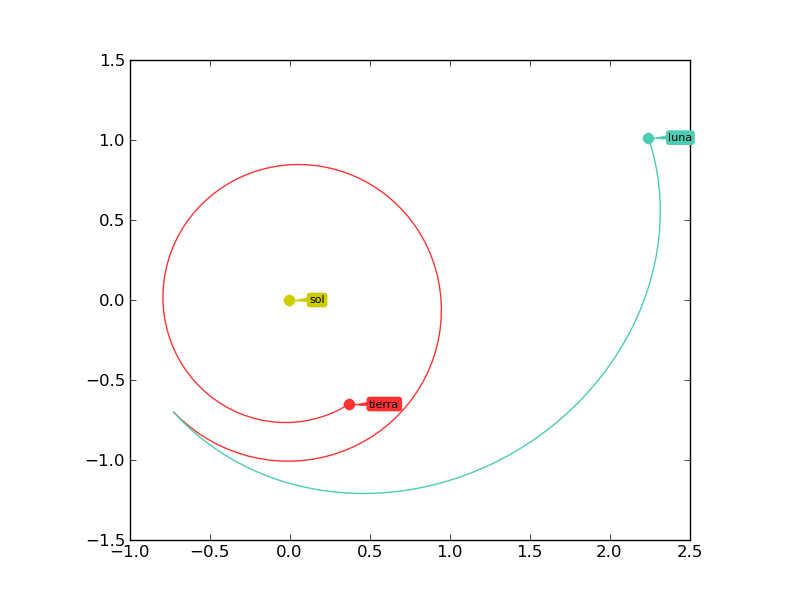
\includegraphics[scale=0.38]{img/ej1/metodo2/validacion_365_1.png}
	\label{fig:ej1_m2_365_1}
	}
	\subfigure[$\delta t$ = 6 horas]{
	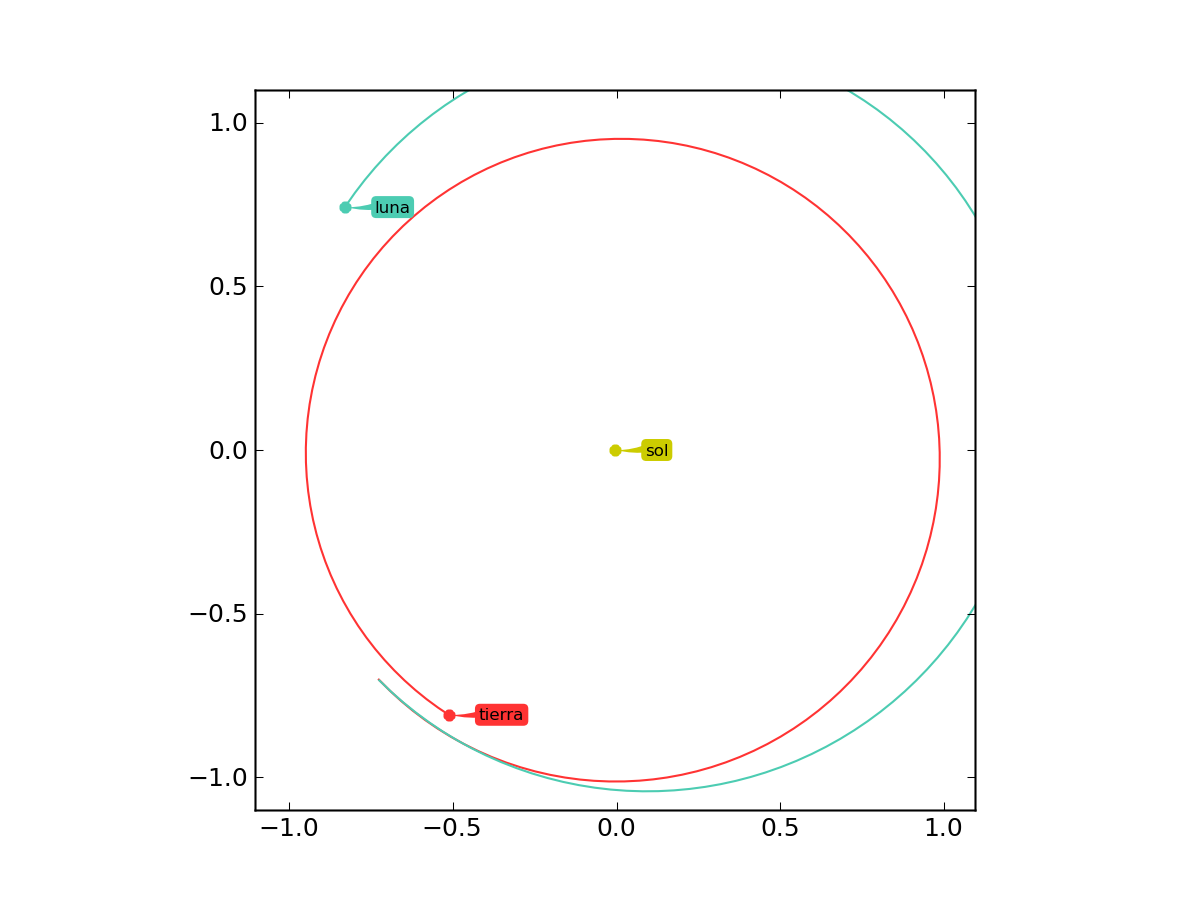
\includegraphics[scale=0.38]{img/ej1/metodo2/validacion_365_4.png}
	\label{fig:ej1_m2_365_4}
	}
	\\
	\subfigure[$\delta t$ = 2 horas]{
	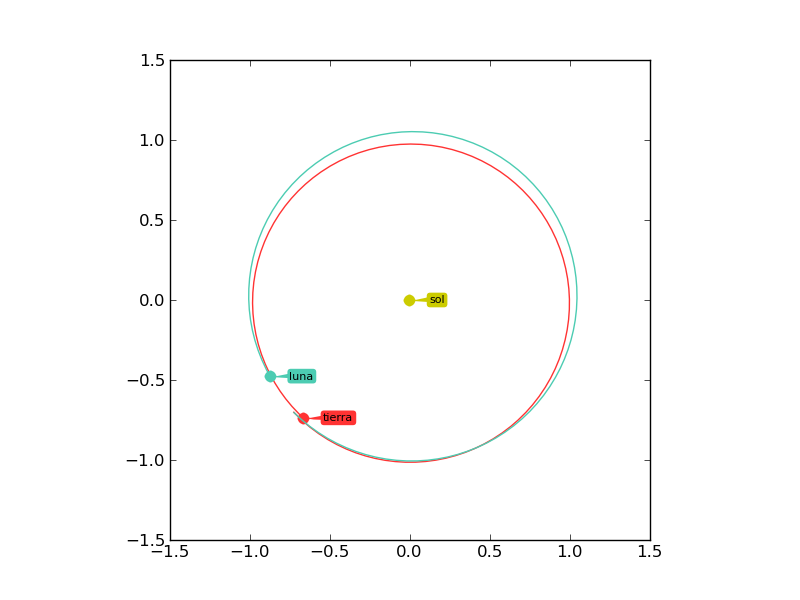
\includegraphics[scale=0.38]{img/ej1/metodo2/validacion_365_12.png}
	\label{fig:ej1_m2_365_12}
	}
	\subfigure[$\delta t$ = 1 hora]{
	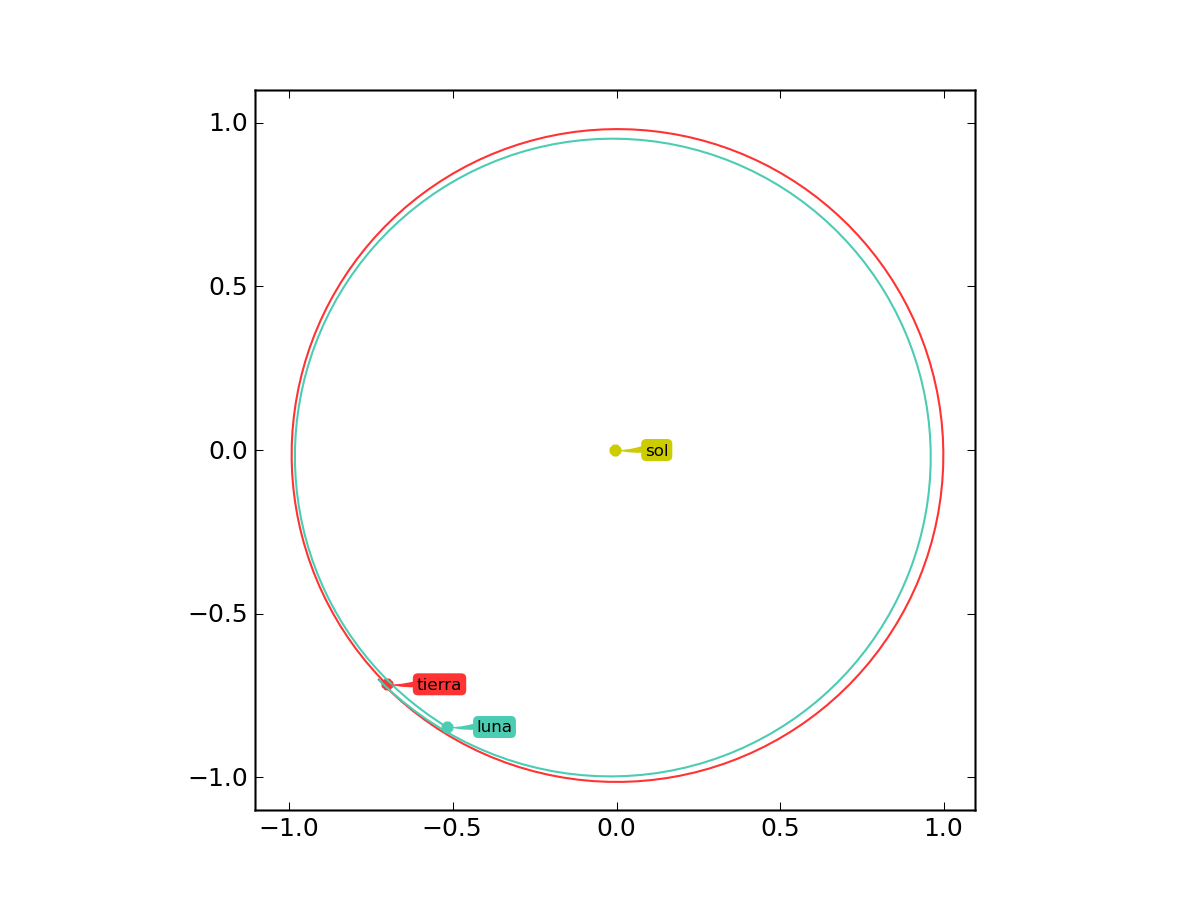
\includegraphics[scale=0.38]{img/ej1/metodo2/validacion_365_24.png}
	\label{fig:ej1_m2_365_24}
	}
	\caption{
		Simulación de validación del sistema sol$-$tierra$-$luna para un período de 1 año y distintos $\delta t$
		con el método 2.
	}
	\label{ fig:res_ej1_m2_365 }
\end{figure}
\begin{figure}
	\centering
	\subfigure[$\delta t$ = 1 día]{
	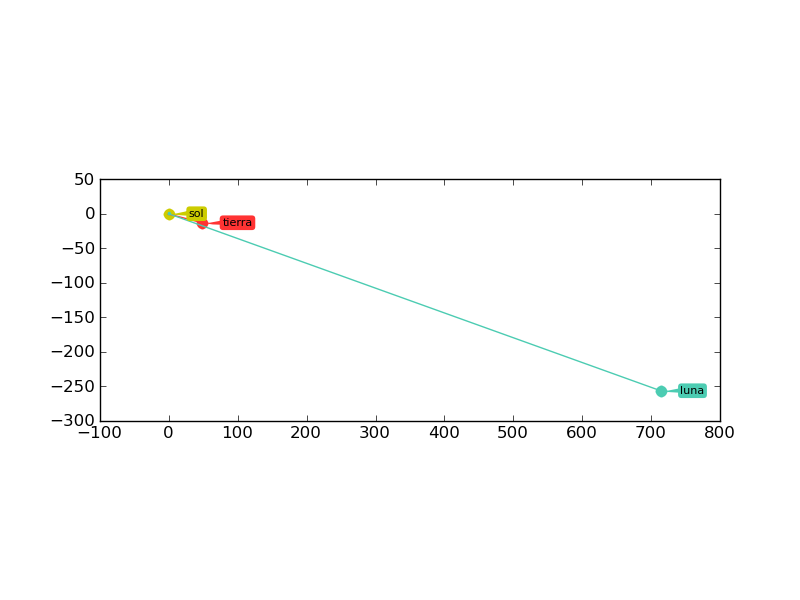
\includegraphics[scale=0.38]{img/ej1/metodo2/validacion_1825_1.png}
	\label{fig:ej1_m2_1825_1}
	}
	\subfigure[$\delta t$ = 6 horas]{
	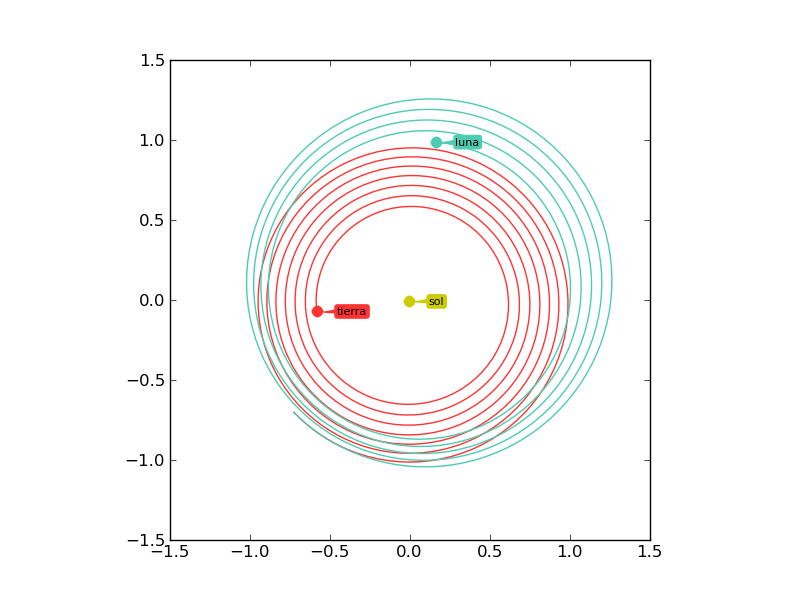
\includegraphics[scale=0.38]{img/ej1/metodo2/validacion_1825_4.png}
	\label{fig:ej1_m2_1825_4}
	}
	\\
	\subfigure[$\delta t$ = 2 horas]{
	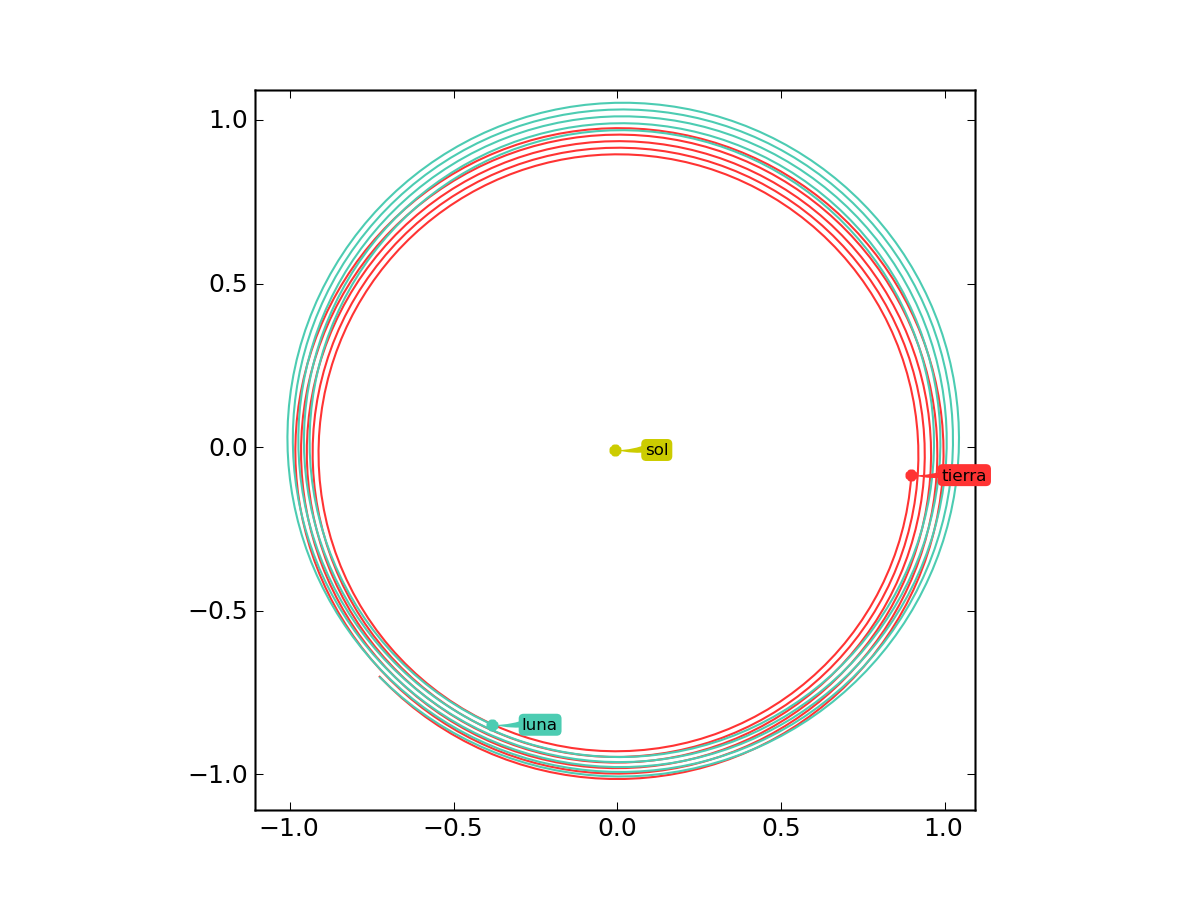
\includegraphics[scale=0.38]{img/ej1/metodo2/validacion_1825_12.png}
	\label{fig:ej1_m2_1825_12}
	}
	\subfigure[$\delta t$ = 1 hora]{
	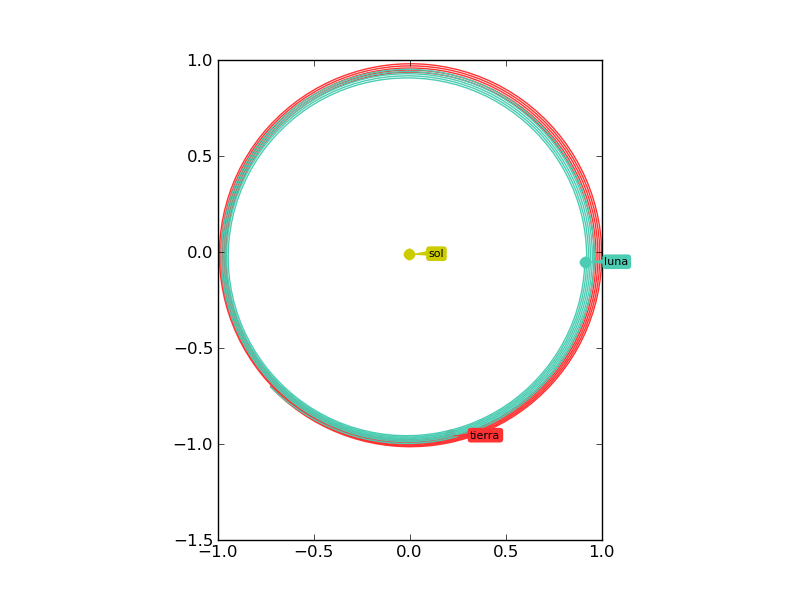
\includegraphics[scale=0.38]{img/ej1/metodo2/validacion_1825_24.png}
	\label{fig:ej1_m2_1825_24}
	}
	\caption{
		Simulación de validación del sistema sol$-$tierra$-$luna para un período de 5 años y distintos $\delta t$
		con el método 2.
	}
	\label{ fig:res_ej1_m2_1825 }
\end{figure}

%		\begin{figure}
	\centering
	\subfigure[$\Delta t$ = 1 día]{
	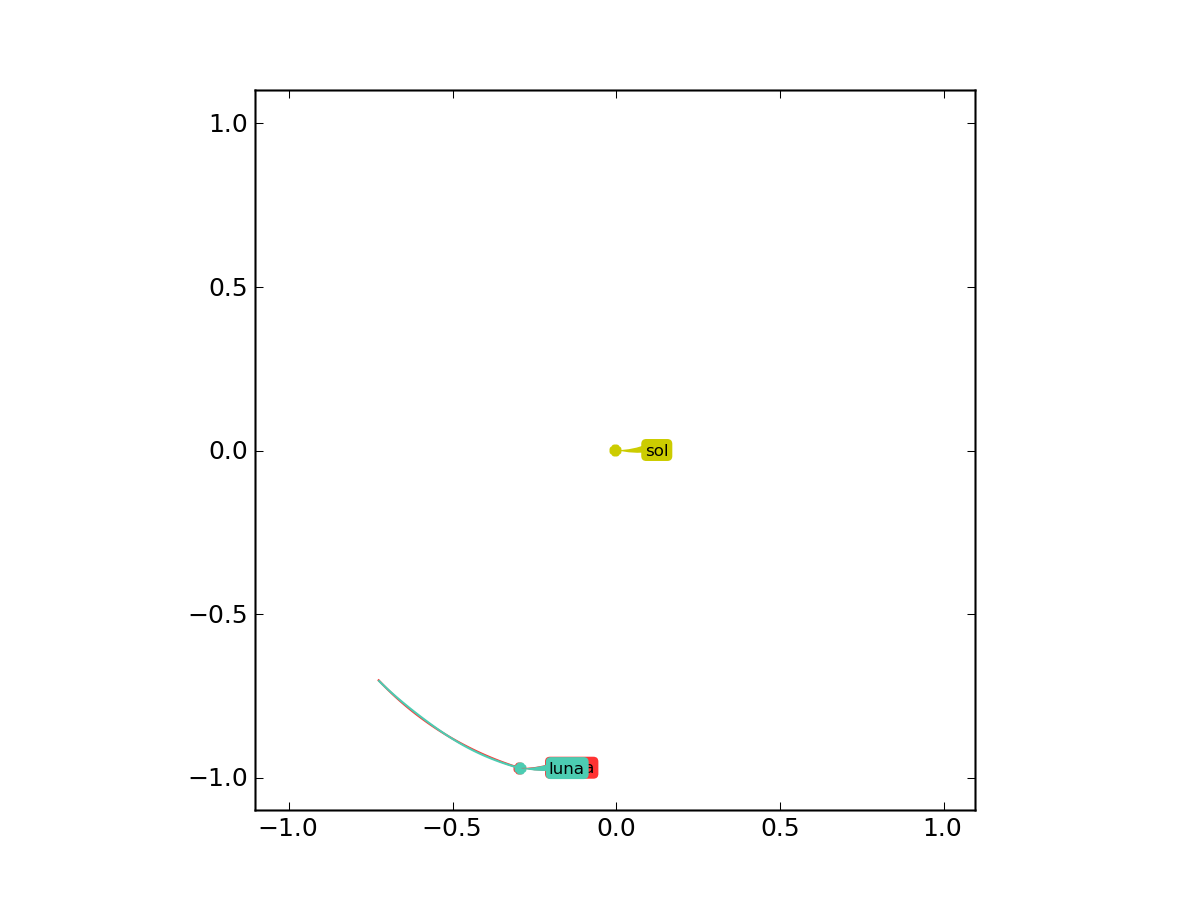
\includegraphics[scale=0.38]{img/ej1/metodo3/validacion_30_1000.png}
	\label{fig:ej1_m3_30_001}
	}
	\\
	\subfigure[$\Delta t$ = 2 horas]{
	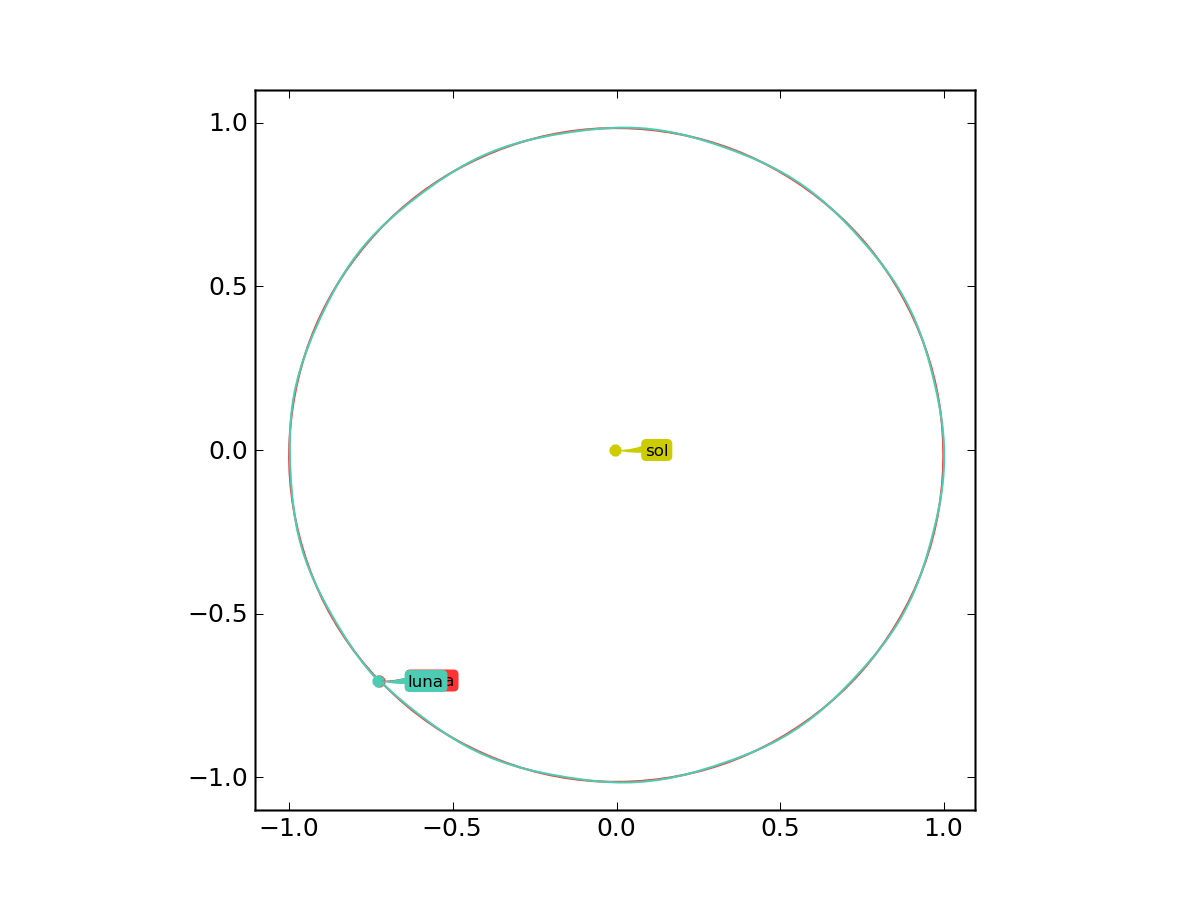
\includegraphics[scale=0.38]{img/ej1/metodo3/validacion_365_1000.png}
	\label{fig:ej1_m3_365_1000}
	}
	\subfigure[$\Delta t$ = 1 hora]{
	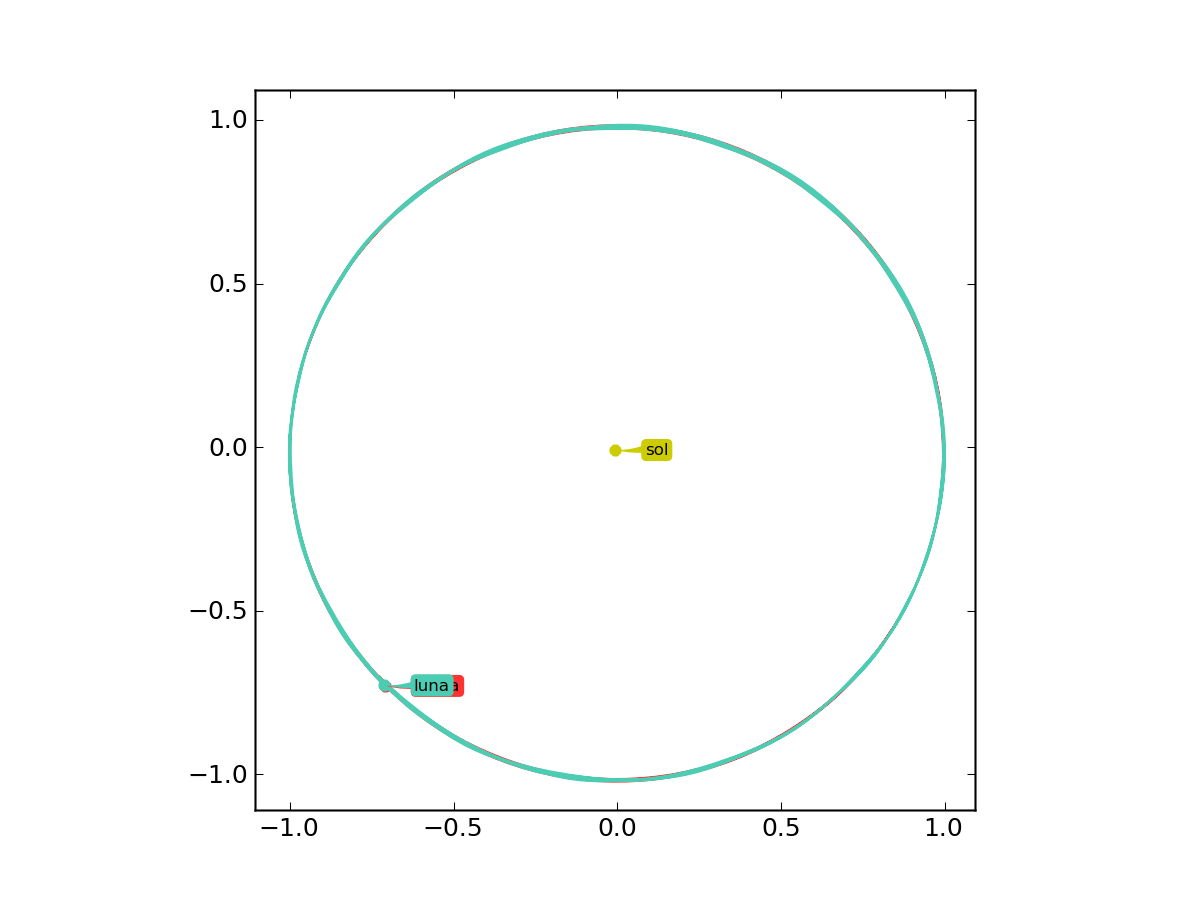
\includegraphics[scale=0.38]{img/ej1/metodo3/validacion_1825_1000.png}
	\label{fig:ej1_m3_1825_1000}
	}
	\caption{
		Simulación de validación del sistema sol$-$tierra$-$luna distintos períodos y un $\Delta t$ de $1/1000$ días
		con el método 3. El método solo funciona bien con $\Delta t$ de este órden o mas chicos.
		Al intentar validar para los $\Delta t$ usados en los otros métodos, no obteníamos resultados razonables.
	}
	\label{ fig:res_ej1_m3 }
\end{figure}

%		\begin{figure}
	\centering
	\subfigure[$\Delta t$ = 1 día]{
	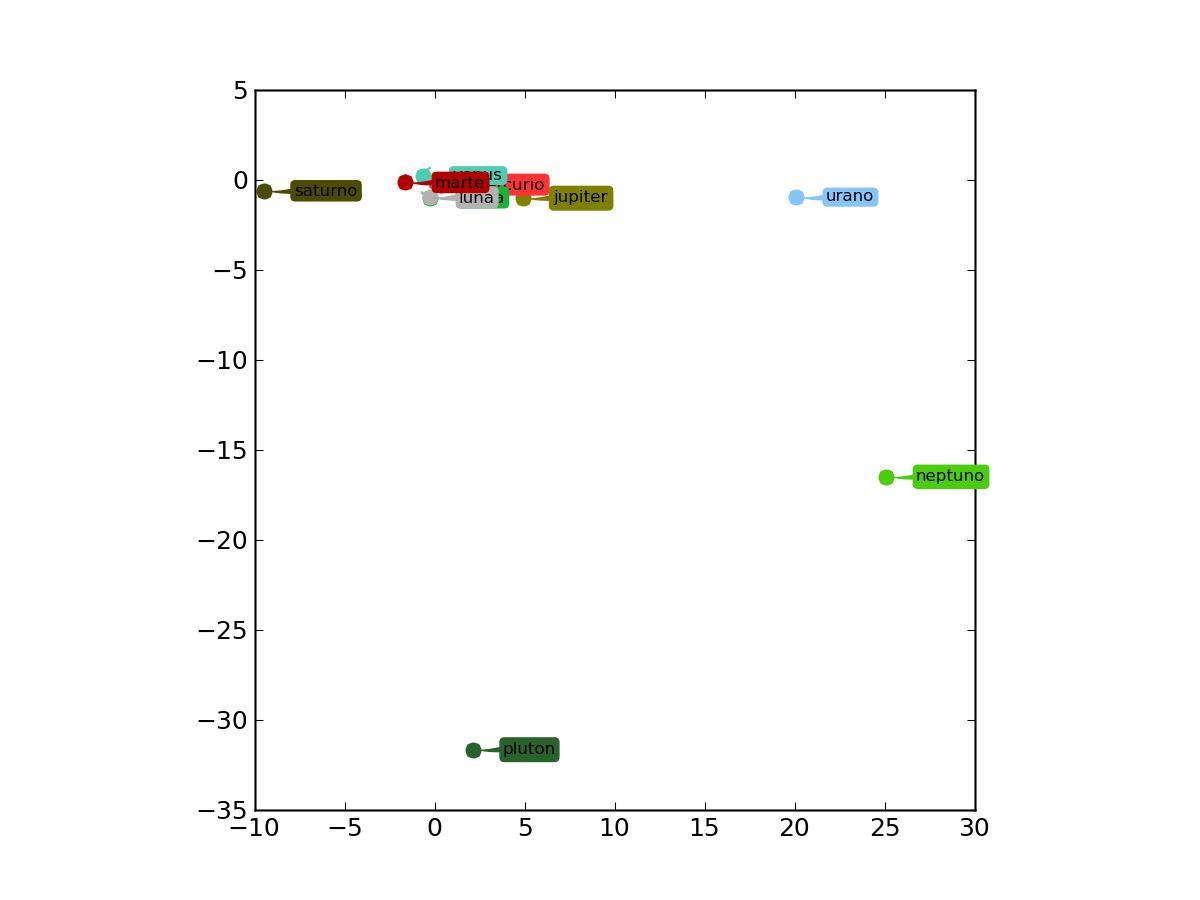
\includegraphics[scale=0.38]{img/ej2/metodo_1/validacion_30_1.png}
	\label{fig:ej2_m1_30_1}
	}
	\subfigure[$\Delta t$ = 6 horas]{
	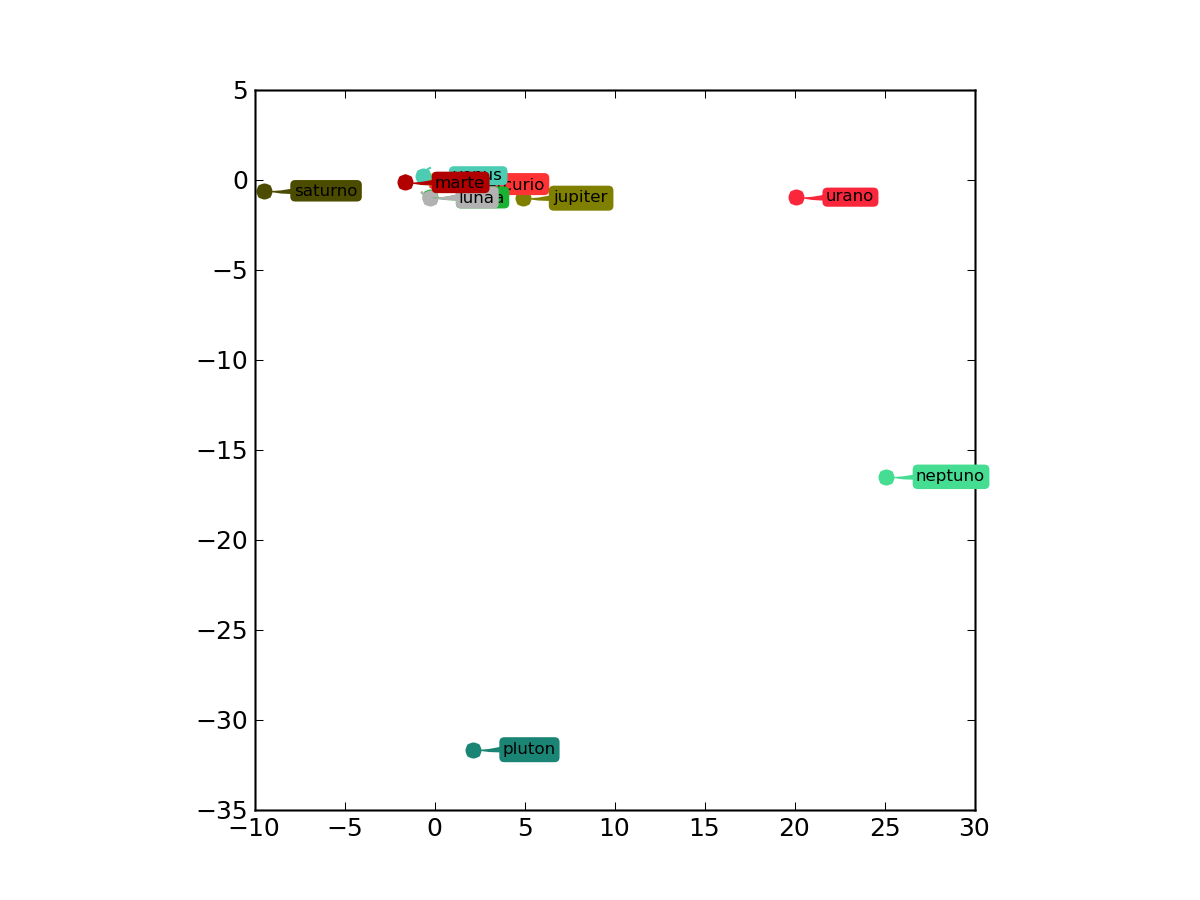
\includegraphics[scale=0.38]{img/ej2/metodo_1/validacion_30_4.png}
	\label{fig:ej2_m1_30_4}
	}
	\\
	\subfigure[$\Delta t$ = 2 horas]{
	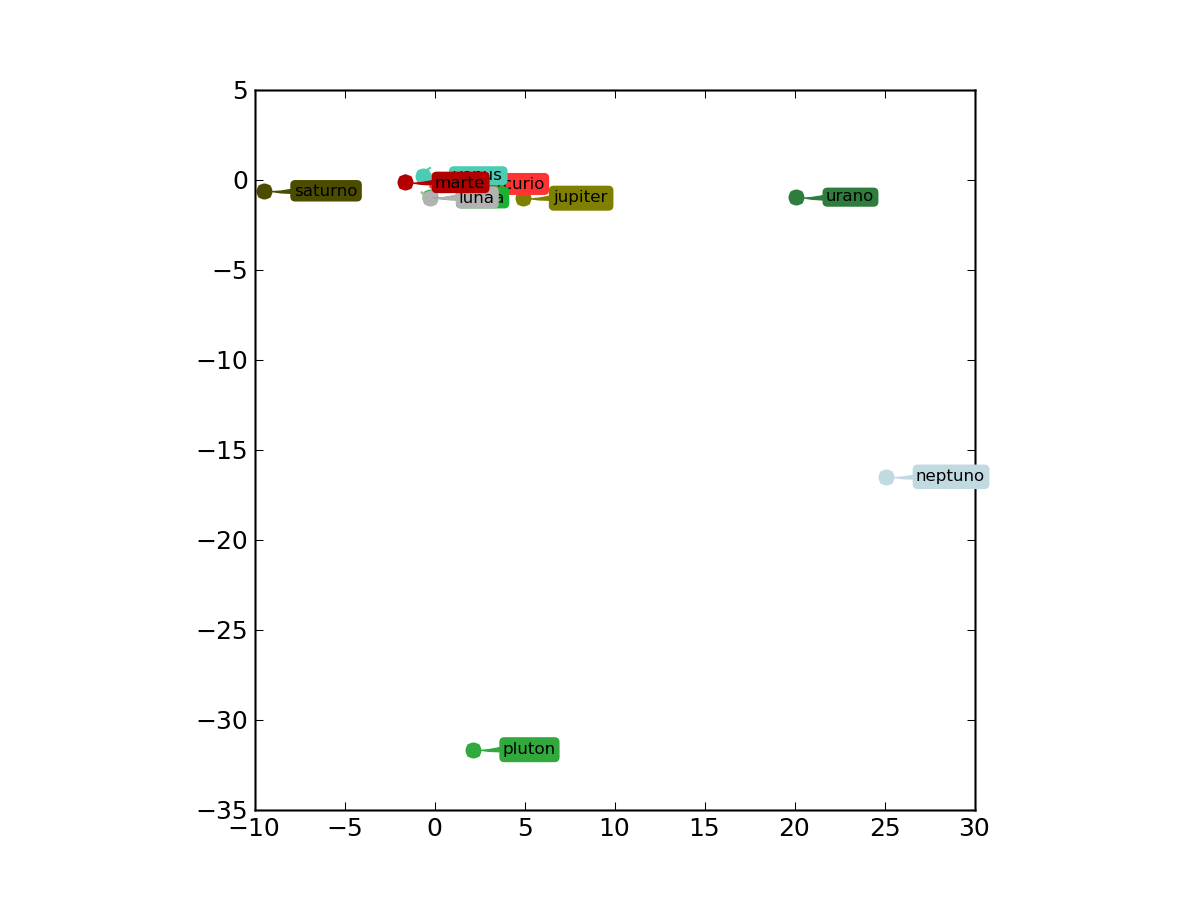
\includegraphics[scale=0.38]{img/ej2/metodo_1/validacion_30_12.png}
	\label{fig:ej2_m1_30_12}
	}
	\subfigure[$\Delta t$ = 1 hora]{
	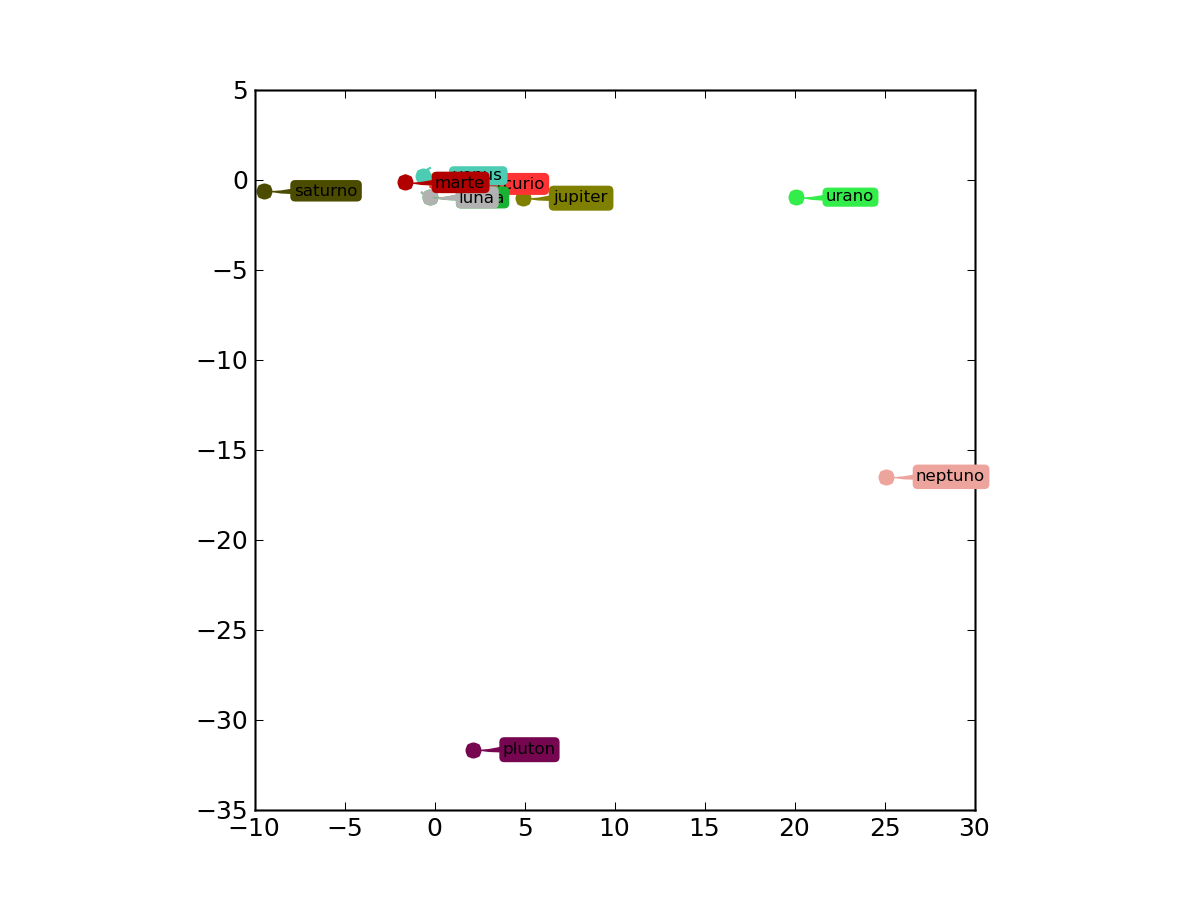
\includegraphics[scale=0.38]{img/ej2/metodo_1/validacion_30_24.png}
	\label{fig:ej2_m1_30_24}
	}
	\caption{
		Simulación de validación del sistema solar para un período de 30 días y distintos $\Delta t$
		con el método 1.
		No hay muchas observaciones que hacer ya que para las dimensiones del sistema solar en 30 días no cambia mucho.
	}
	\label{ fig:res_ej2_m1_30 }
\end{figure}
\begin{figure}
	\centering
	\subfigure[$\Delta t$ = 1 día]{
	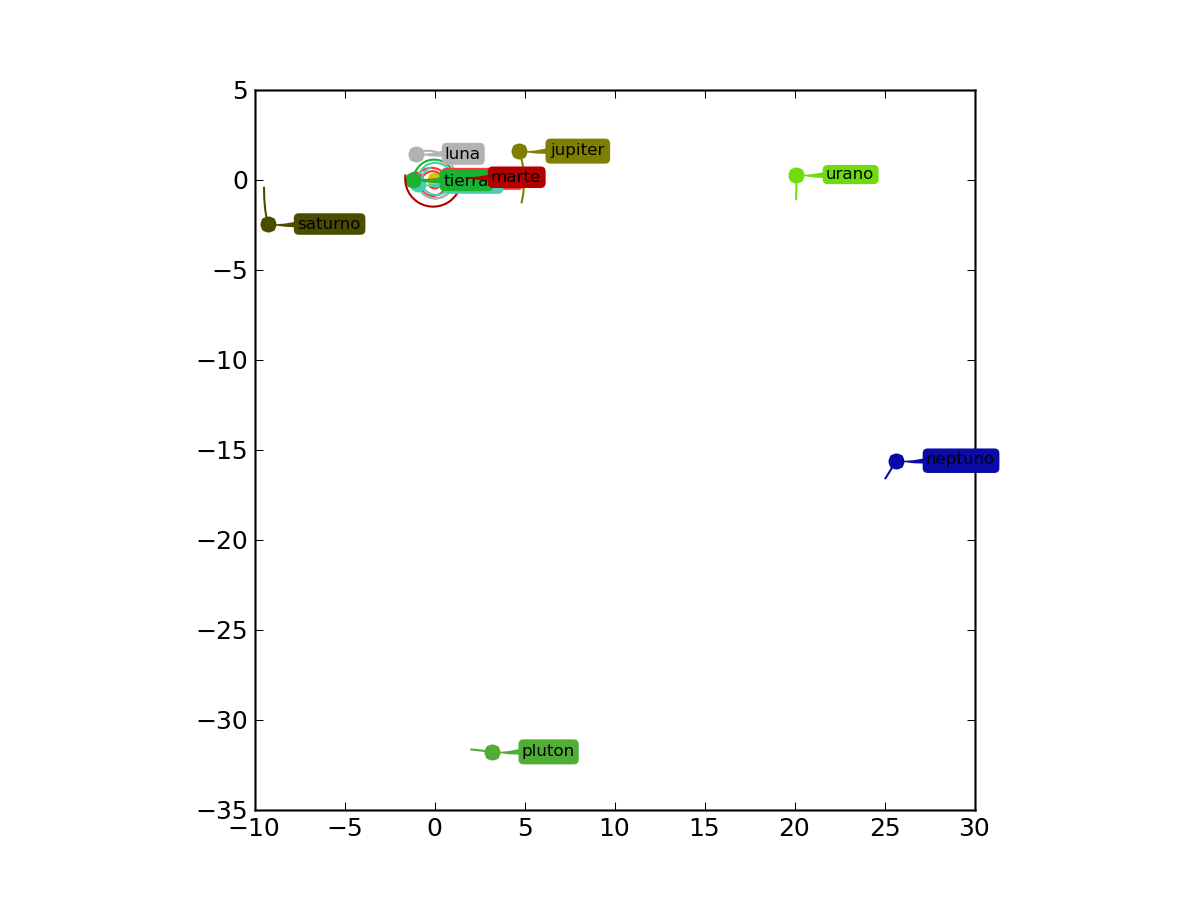
\includegraphics[scale=0.38]{img/ej2/metodo_1/validacion_365_1.png}
	\label{fig:ej2_m1_365_1}
	}
	\subfigure[$\Delta t$ = 6 horas]{
	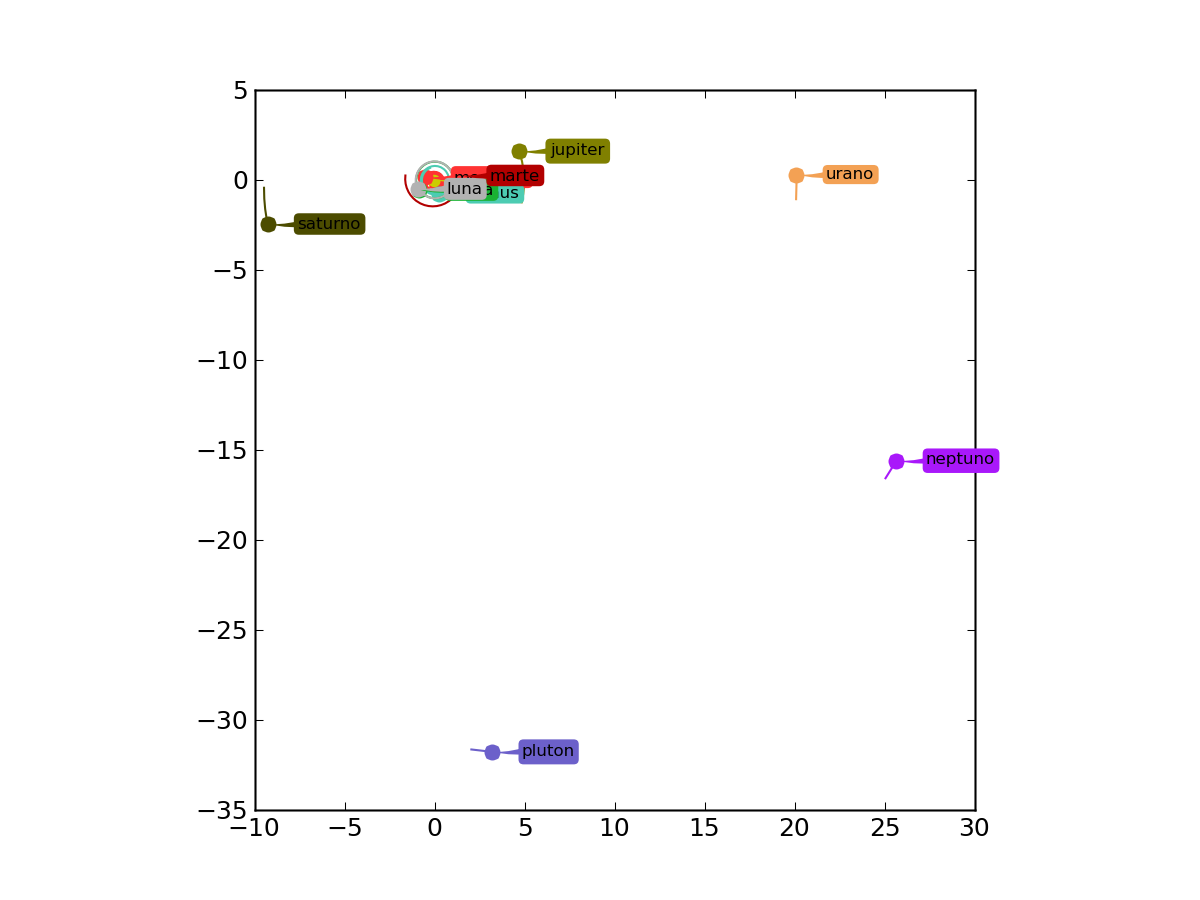
\includegraphics[scale=0.38]{img/ej2/metodo_1/validacion_365_4.png}
	\label{fig:ej2_m1_365_4}
	}
	\\
	\subfigure[$\Delta t$ = 2 horas]{
	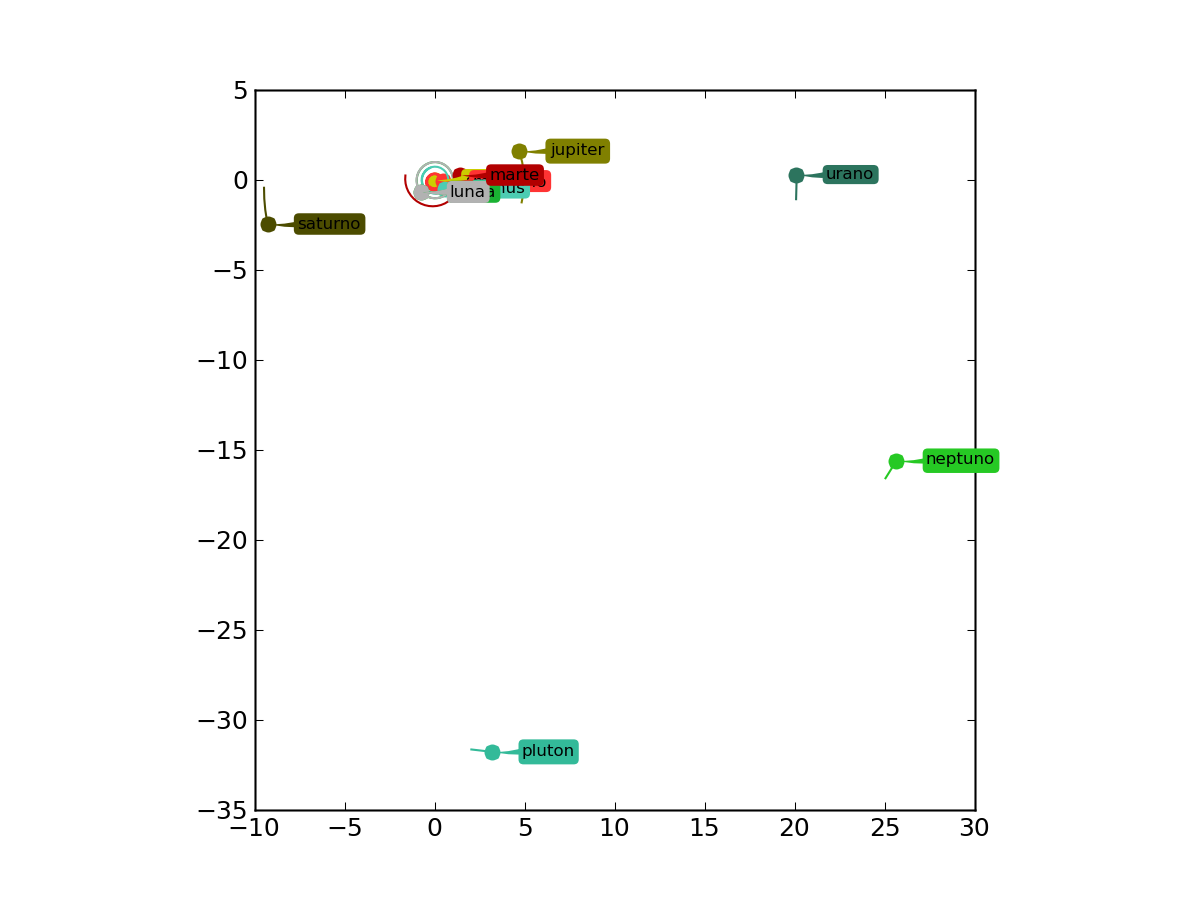
\includegraphics[scale=0.38]{img/ej2/metodo_1/validacion_365_12.png}
	\label{fig:ej2_m1_365_12}
	}
	\subfigure[$\Delta t$ = 1 hora]{
	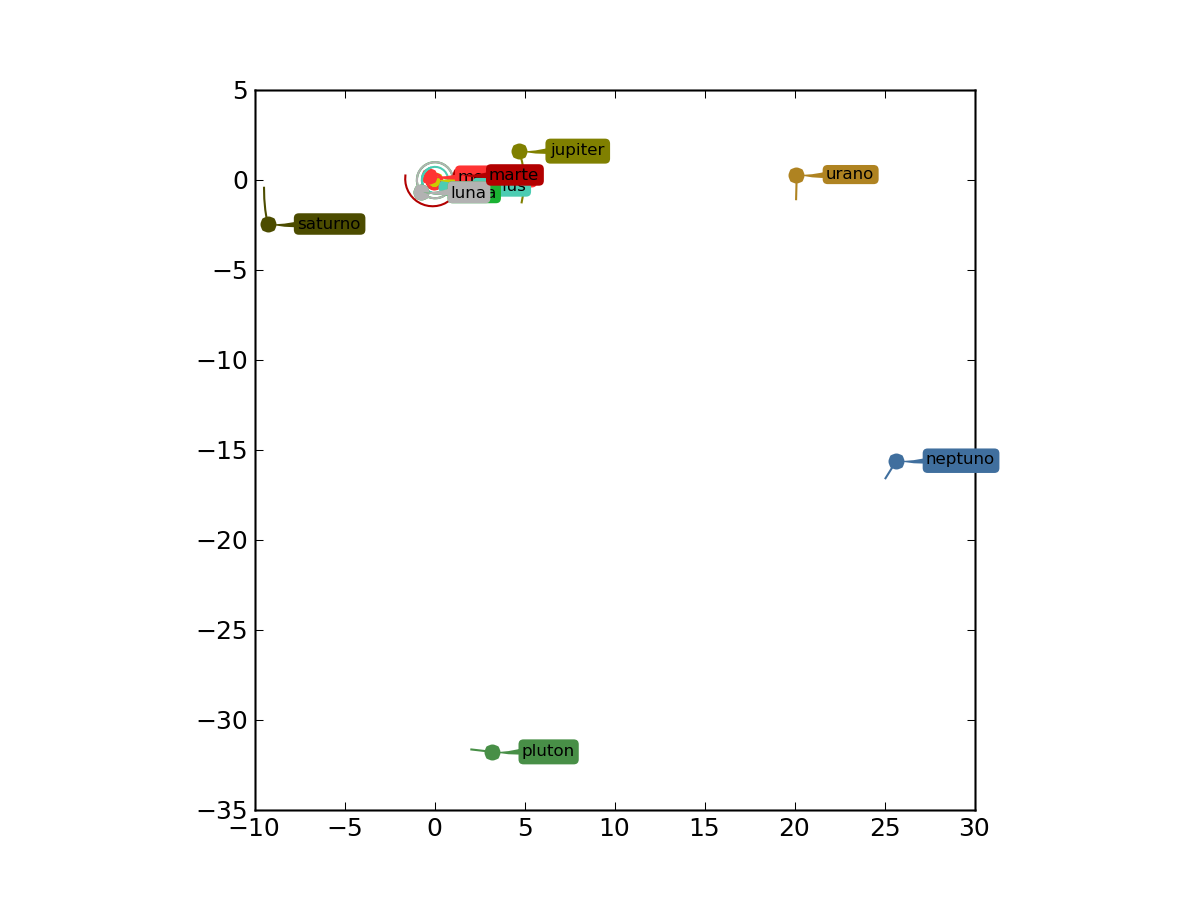
\includegraphics[scale=0.38]{img/ej2/metodo_1/validacion_365_24.png}
	\label{fig:ej2_m1_365_24}
	}
	\caption{
		Simulación de validación del sistema solar para un período de 1 año y distintos $\Delta t$
		con el método 1.
		Vemos que las órbitas de los planetas del ejercicio anterior se siguen comportando bien,
		lo que era de esperarse ya que los planetas que agregamos no deberían influenciar demasiado sus órbitas, por estar muy distanciados.
	}
	\label{ fig:res_ej2_m1_365 }
\end{figure}
\begin{figure}
	\centering
	\subfigure[$\Delta t$ = 1 día]{
	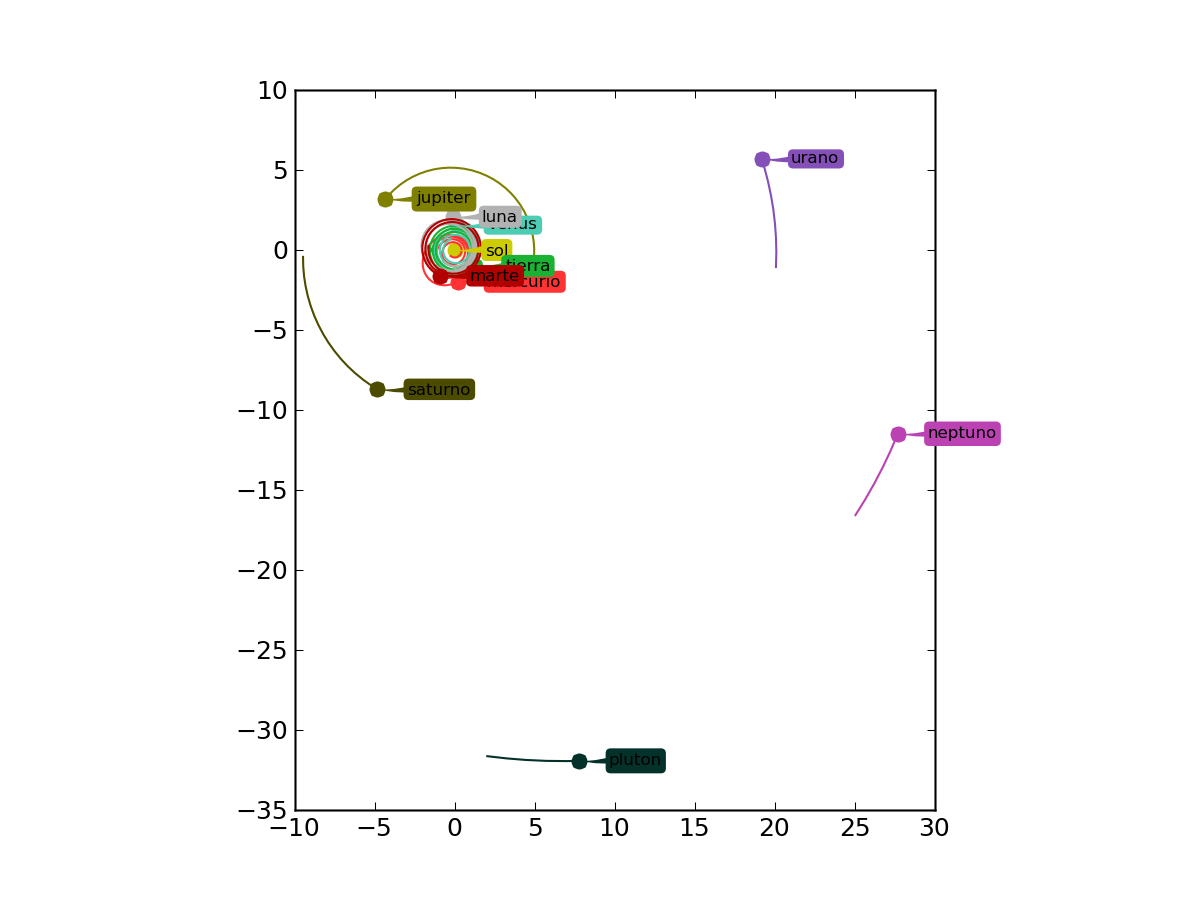
\includegraphics[scale=0.38]{img/ej2/metodo_1/validacion_1825_1.png}
	\label{fig:ej2_m1_1825_1}
	}
	\subfigure[$\Delta t$ = 6 horas]{
	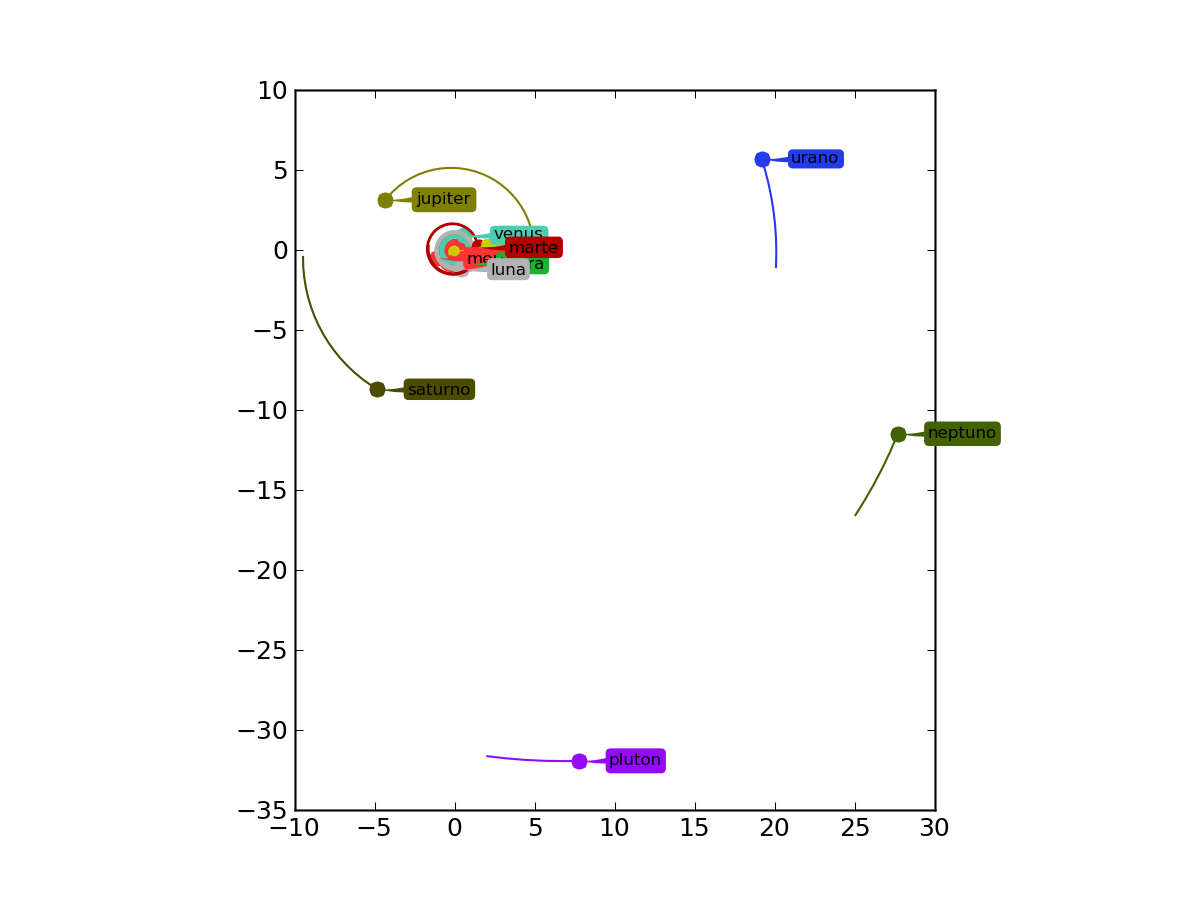
\includegraphics[scale=0.38]{img/ej2/metodo_1/validacion_1825_4.png}
	\label{fig:ej2_m1_1825_4}
	}
	\\
	\subfigure[$\Delta t$ = 2 horas]{
	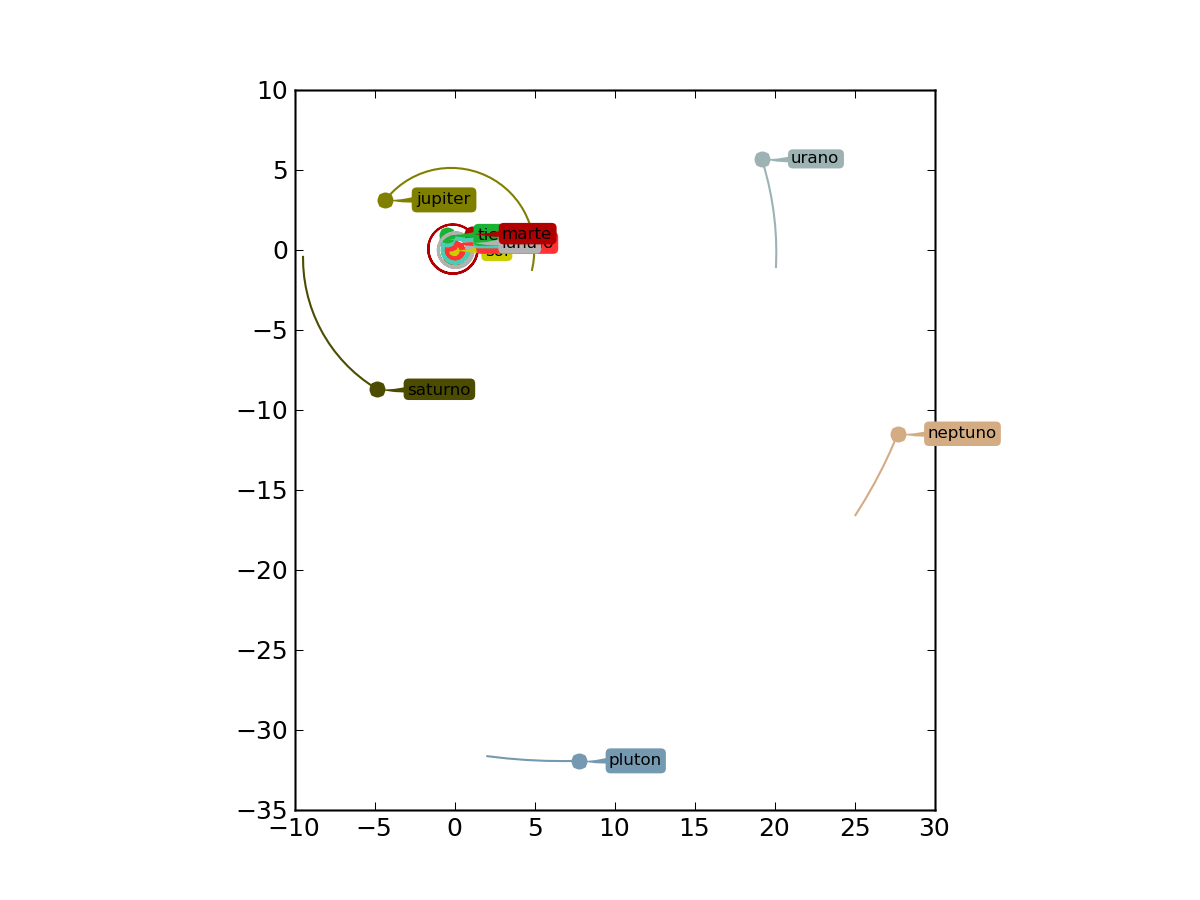
\includegraphics[scale=0.38]{img/ej2/metodo_1/validacion_1825_12.png}
	\label{fig:ej2_m1_1825_12}
	}
	\subfigure[$\Delta t$ = 1 hora]{
	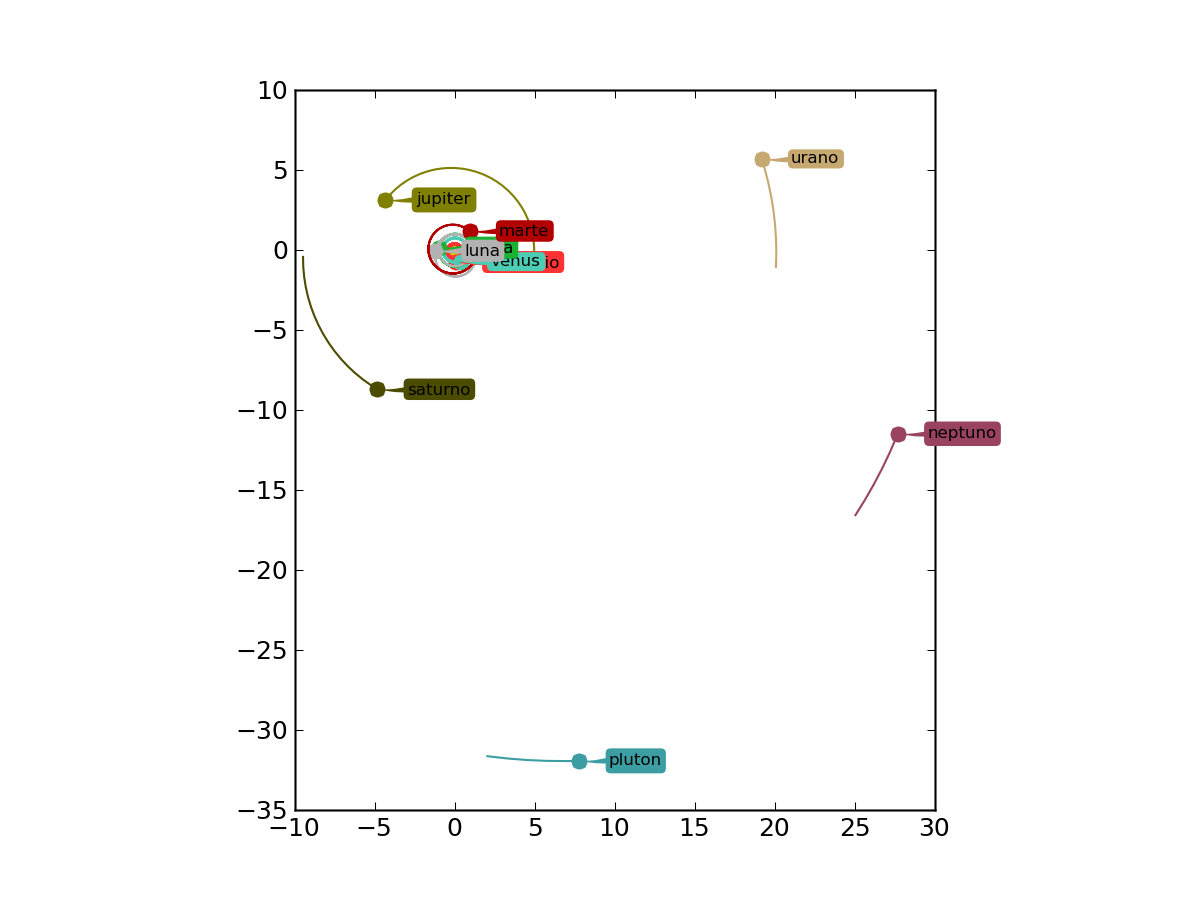
\includegraphics[scale=0.38]{img/ej2/metodo_1/validacion_1825_24.png}
	\label{fig:ej2_m1_1825_24}
	}
	\caption{
		Simulación de validación del sistema solar para un período de 5 años y distintos $\Delta t$
		con el método 1.
		No vemos cambios mayores a simple vista a esta escala,
		lo que indica que para las dimensiónes del sistema solar,
		las simulaciónes de las órbitas mas grandes son razonables también con $\Delta t$ mas chicos para este período
		(depende de que precisión se este buscando).
	}
	\label{ fig:res_ej2_m1_1825 }
\end{figure}

%		\begin{figure}
	\centering
	\subfigure[$\delta t$ = 1 día]{
	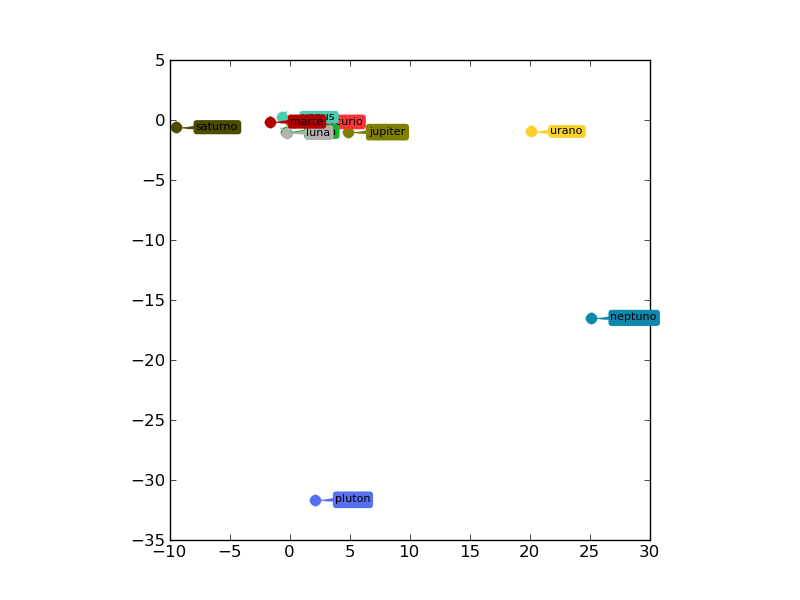
\includegraphics[scale=0.38]{img/ej2/metodo_2/validacion_30_1.png}
	\label{fig:ej2_m2_30_1}
	}
	\subfigure[$\delta t$ = 6 horas]{
	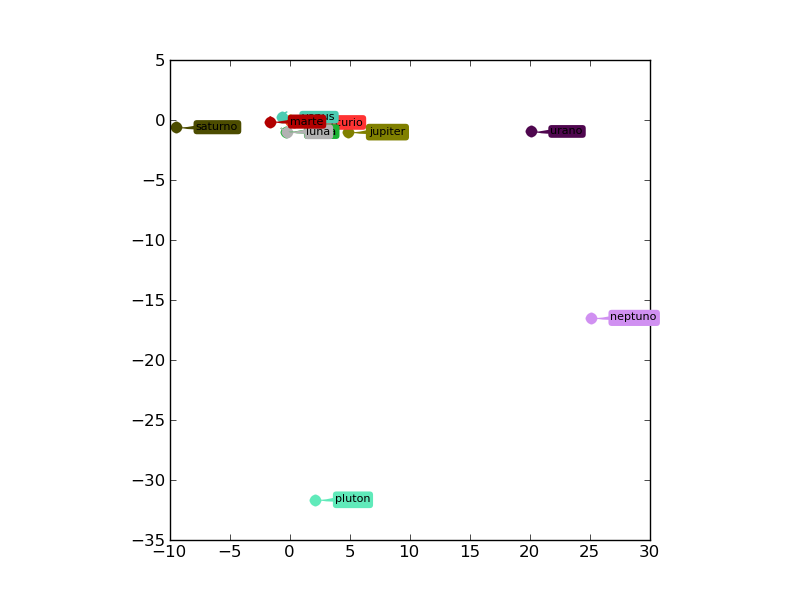
\includegraphics[scale=0.38]{img/ej2/metodo_2/validacion_30_4.png}
	\label{fig:ej2_m2_30_4}
	}
	\\
	\subfigure[$\delta t$ = 2 horas]{
	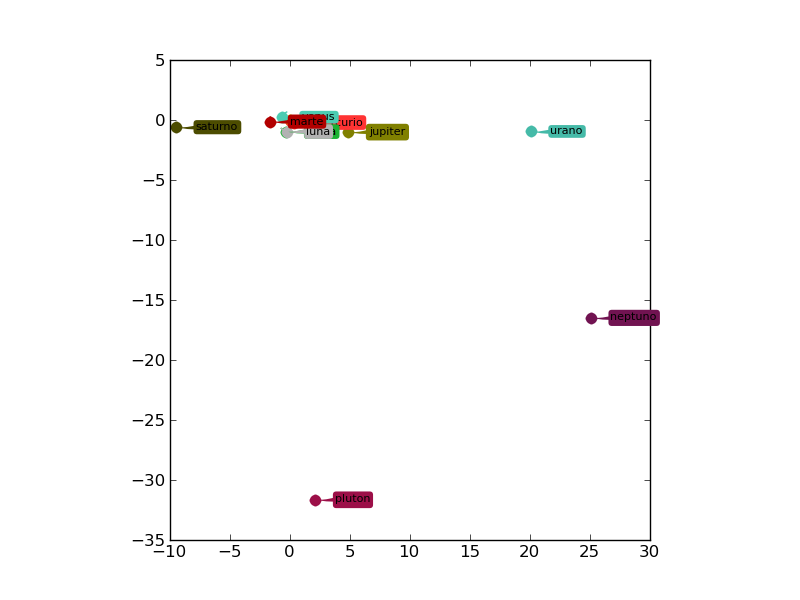
\includegraphics[scale=0.38]{img/ej2/metodo_2/validacion_30_12.png}
	\label{fig:ej2_m2_30_12}
	}
	\subfigure[$\delta t$ = 1 hora]{
	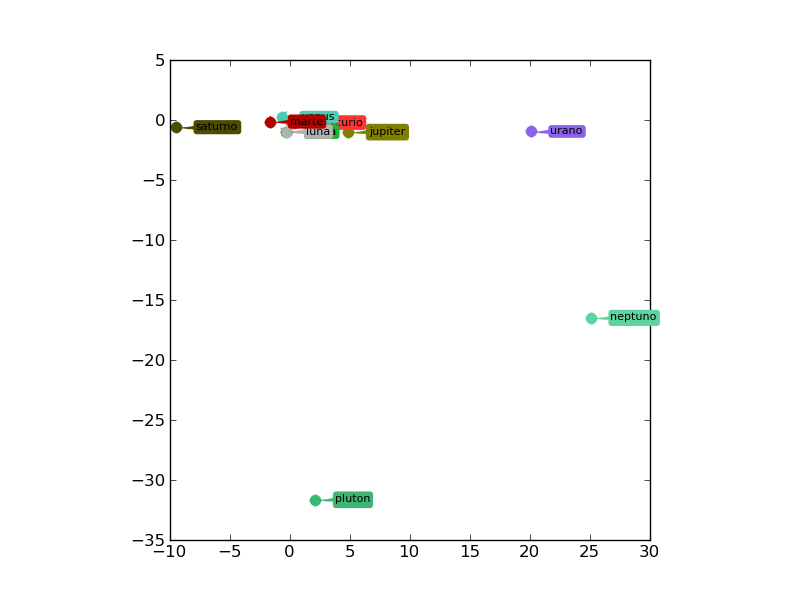
\includegraphics[scale=0.38]{img/ej2/metodo_2/validacion_30_24.png}
	\label{fig:ej2_m2_30_24}
	}
	\caption{
		Simulación de validación del sistema solar para un período de 30 días y distintos $\delta t$
		con el método 2.
		Observamos que el error no parece ser tan grande a simple vista para este período.
	}
	\label{ fig:res_ej2_m2_30 }
\end{figure}
\begin{figure}
	\centering
	\subfigure[$\delta t$ = 1 día]{
	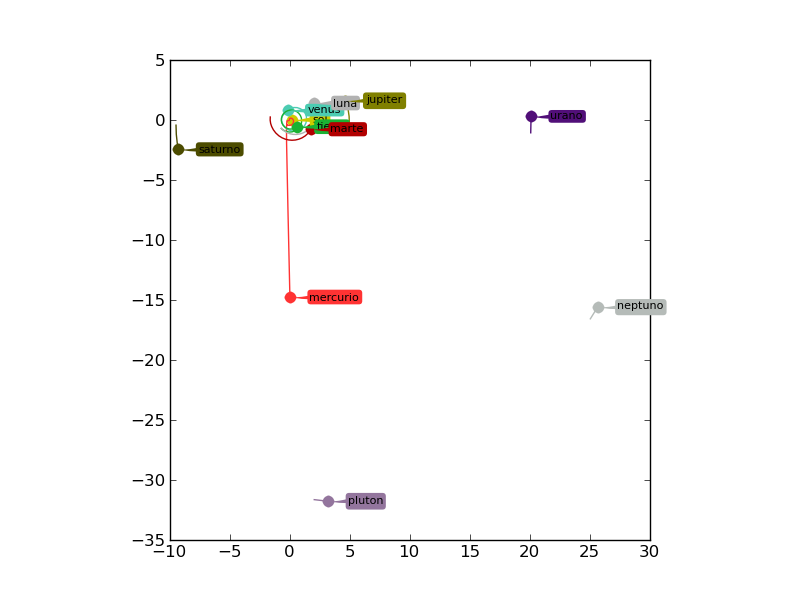
\includegraphics[scale=0.38]{img/ej2/metodo_2/validacion_365_1.png}
	\label{fig:ej2_m2_365_1}
	}
	\subfigure[$\delta t$ = 6 horas]{
	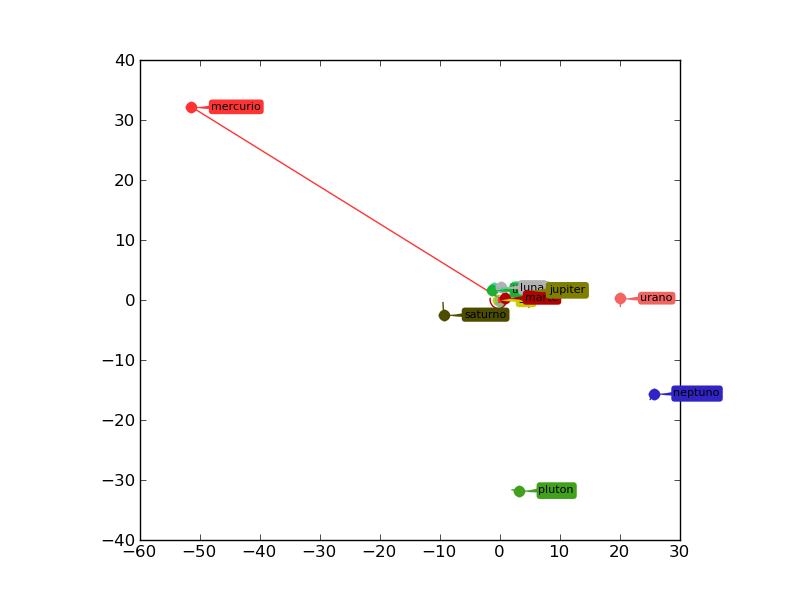
\includegraphics[scale=0.38]{img/ej2/metodo_2/validacion_365_4.png}
	\label{fig:ej2_m2_365_4}
	}
	\\
	\subfigure[$\delta t$ = 2 horas]{
	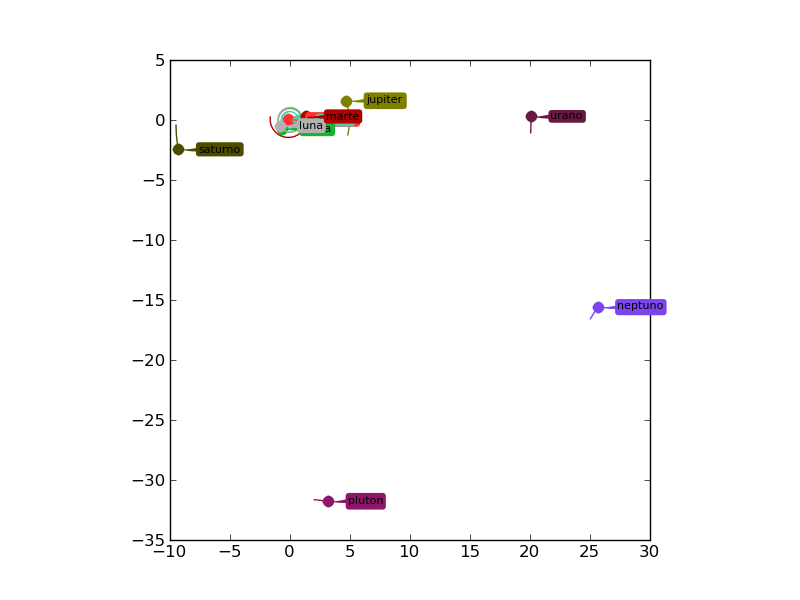
\includegraphics[scale=0.38]{img/ej2/metodo_2/validacion_365_12.png}
	\label{fig:ej2_m2_365_12}
	}
	\subfigure[$\delta t$ = 1 hora]{
	\includegraphics[scale=0.38]{img/ej2/metodo_2/validacion_365_24.png}
	\label{fig:ej2_m2_365_24}
	}
	\caption{
		Simulación de validación del sistema solar para un período de 1 año y distintos $\delta t$
		con el método 2.
		Para esta cantidad de tiempo, la simulación con un $\delta t$ de un día ya merece ser descartada.
		Las otras todavía parecen comportarse razonablemente
	}
	\label{ fig:res_ej2_m2_365 }
\end{figure}
\begin{figure}
	\centering
	\subfigure[$\delta t$ = 1 día]{
	\includegraphics[scale=0.38]{img/ej2/metodo_2/validacion_1825_1.png}
	\label{fig:ej2_m2_1825_1}
	}
	\subfigure[$\delta t$ = 6 horas]{
	\includegraphics[scale=0.38]{img/ej2/metodo_2/validacion_1825_4.png}
	\label{fig:ej2_m2_1825_4}
	}
	\\
	\subfigure[$\delta t$ = 2 horas]{
	\includegraphics[scale=0.35]{img/ej2/metodo_2/validacion_1825_12.png}
	\label{fig:ej2_m2_1825_12}
	}
	\subfigure[$\delta t$ = 1 hora]{
	\includegraphics[scale=0.35]{img/ej2/metodo_2/validacion_1825_24.png}
	\label{fig:ej2_m2_1825_24}
	}
	\caption{
		Simulación de validación del sistema solar para un período de 5 años y distintos $\delta t$
		con el método 2.
		Para esta cantidad de tiempo de simulación, las órbitas de los planetas ya comienzan a mostrar error al dar más de una vuelta.
		El mejor método parece ser el de $\delta t$ de 2 horas, ya que para el de 1 hora la luna comienza a comportarse de una manera un poco mas extraña.
	}
	\label{ fig:res_ej2_m2_1825 }
\end{figure}

%		\begin{figure}
	\centering
	\subfigure[Impacto zoom: all]{
	\includegraphics[scale=0.38]{img/torpedo/proyectilhit_all.png}
	\label{fig:res_misil_1}
	}
	\\
	\subfigure[Impacto zoom: 2.2]{
	\includegraphics[scale=0.38]{img/torpedo/proyectilhit_zoom1.png}
	\label{fig:res_misil_2}
	}
	\subfigure[Impacto zoom: .2]{
	\includegraphics[scale=0.38]{img/torpedo/proyectilhit_zoom2.png}
	\label{fig:res_misil_3}
	}
	\caption{
		Acá vemos la simulación de el proyectil \textit{Torpedo de Protones} para una instancia en la que le pega a la tierra,
		con distintas ampliaciones.
		El misil fue disparado desde el punto $<-30,.005, 0>$ (aproximadamente) a una velocidad de $<0.147774,0.00480309,-3.62451e-08>$ AU/día.
	}
	\label{ fig:res_misil }
\end{figure}

%		\begin{figure}
	\centering
	\subfigure[Impacto zoom: all]{
	\includegraphics[scale=0.38]{img/bomba/bombaoscurahit_all.png}
	\label{fig:res_bomba_1}
	}
	\subfigure[Impacto zoom: 2.2]{
	\includegraphics[scale=0.38]{img/bomba/bombaoscurahit_zoom1.png}
	\label{fig:res_bomba_2}
	}
	\\
	\subfigure[Impacto zoom: .2]{
	\includegraphics[scale=0.38]{img/bomba/bombaoscurahit_zoom2.png}
	\label{fig:res_bomba_3}
	}
	\subfigure[intento de impacto]{
	\includegraphics[scale=0.38]{img/bomba/decote.png}
	\label{fig:res_bomba_4}
	}
	\caption{
		Acá vemos la simulación de el proyectil \textit{Bomba Oscura} para una instancia en la que le pega a la tierra,
		con distintas ampliaciones.
		El misil fue disparado desde el punto $<0,30,0>$ AU (aproximadamente) a una velocidad de $<0.00150022,-0.0346204,0>$ AU/día.
		En la última imagen vemos un intento de pegarle a la tierra bastante rebuscado, que paso muy cerca de su objetivo.
		Esto nos muestra que hay muchísimas posibilidades extrañas también de pegarle a la tierra pero que requieren de un cálculo mucho mas fino ya que
		aparecen distancias chicas que vuelven al sistema bastante inestable numericamente.
	}
	\label{ fig:res_bomba }
\end{figure}

	\end{usection}
	
	\begin{usection}{Discusión}
		
		
		\begin{usubsection}{Algoritmo de búsqueda del mínimo \texttt{mindist}}
		Para cada trayectoria inicial, definimos una grilla de $3 \times 3$
		puntos, donde el punto central era ella misma, y los otros
		puntos son las rotaciones de la velocidad sobre los ejes
		anteriormente mencionados por dos ángulos, respectivamente, de
		un módulo inicial que se reduce a la mitad en cada iteración de
		la búsqueda, y luego disparámos proyectiles en todas las 9
		direcciónes.
		Así, aunque en algunos casos asintóticamente,
		podemos llegar a cualquier punto del espacio
		contenido en la grilla inicial (la definida en la primera
		iteración) si alli se encuentra una solución.
		A la grilla inicial le ponemos un ancho inicial grosero, de
		manera de incluír casi necesariamente a alguna solución.

		\begin{figure}[H]
			\centering
			\includegraphics[scale=0.5]{img/grid.png}
			\caption{
				En la imagen vemos una representación gráfica de los
				sucesivos espacios de búsqueda local. el orden de las
				iteraciones es rojo $\rightarrow$ azul
				$\rightarrow$ verde.
			}
			\label{fig:grilla}
		\end{figure}		

		Para elegir la trayectoria inicial del algoritmo, calculamos
		primero aproximadamente (simulando y visualizando) cuanto
		tiempo tardaba el proyectil en llegar hasta la órbita terrestre
		desde la órbita de neptuno. Luego calculamos aproximadamente
		la posición de la Tierra en esa cantidad de tiempo después de la
		fecha inicial de lanzamiento, tomando los datos de la posición
		de ese día de la información que provee la NASA.

		También de esos datos, elegimos un punto arbitrario en la
		órbita de Neptuno para el lanzamiento del proyectil. Como
		dirección de la velocidad inicial del proyectil, elegimos el
		vector resultante de restar la posición inicial del proyectil a la
		posición aproximada del impacto sobre la órbita terrestre.
		El módulo de la velocidad inicial, es el propuesto por el
		enunciado del problema.

		Luego de probar para un par de posiciones y velocidades
		iniciales distintas, encontramos soluciones donde pudimos
		destruír la tierra. Las mismas están detalladas en la sección
		siguiente.
		\end{usubsection}
		
		\begin{usubsection}{Gauss}
			Elegimos resolver los sistemas lineales usando el método de Gauss porque es fácil de implementar y es un poco más eficiente que los métodos de factorización.
			No se justifica usar \texttt{LU} porque la ventaja principal es que hay que factorizar la matriz una sola vez para resolver muchos sistemas, pero nosotros resolvemos siempre sistemas con diferentes matrices.
		\end{usubsection}

		\begin{usubsection}{$\Delta t$}
			Un problema que observamos durante las simulaciones, cuando tratábamos de pegarle con el proyectil a la tierra, es que el $\Delta t$ no era lo suficientemente chico para lograr la presicion de impacto requerida.
			De un instante de tiempo al otro, el proyectil estaba adelante y luego atrás de la tierra, siendo la distancia entre los cuerpos nunca suficientemente chica.
			Por esto en la función \texttt{mindist} alteramos el $\Delta t$ dinámicamente a medida que el proyectil se acercaba al \texttt{target}, para tener más presicion cuando se encontraban cerca.
		\end{usubsection}
		
	\end{usection}
	
	\begin{section}*{Conclusiones}	\addcontentsline{toc}{section}{Conclusiones}

		Llegamos a la conclusión que, dados los métodos implementados,
		el mejor en la práctica para el ejercicio de destruír la tierra, resulto ser el método 1, ya que,
		los otros solo resultaban muy buenos (mejores incluso en cuanto a los resultados finales que el método 1)
		si el $\Delta t$ era significativamente muy bajo,
		lo que para nuestro algoritmo de búsqueda local era muy malo en cuanto a tiempo de ejecución.

		No obstante, más alla de la sensibilidad del método 2 a los $\Delta t$ altos,
		el método de triangulación resulto ser bastante mas rápido de lo que esperabamos, en la práctica.

		Un detalle que notamos fue que la precisión relativa entre el método 1 y 2 de la simulación, a medida que el $\Delta t$ se iba haciendo mas chico,
		era muy similar. Lo que concluímos fue que a pesar de que los 2 algoritmos son bastante distintos,
		y el segundo pareciera ser mucho más sofisticado, las aproximaciones que hacemos en ambos casos son siempre lineales,
		lo que parece justificar nuestras observaciones sobre la similitud de los métodos antes mencionada,
		y nos dice que a partir de un cierto $\Delta t$ suficientemente chico (ya que el método 2 es mas sensible con $\Delta t$ grande) las aproximaciónes del segundo método
		no van a ser mejores que las del primero.

		El método 3 parece arreglar este problema, aproximando varias derivadas en un mismo $\Delta t$,
		hasta que la diferencia entre dos derivadas sucesivas se haga mas chica que un umbral.
		Sin embargo esto es muy parecido, y practicamente igual de eficiente que achicar todavía mas el $\Delta t$ para los métodos anteriores.
		

	\end{section}
	
	\begin{usection}{Apéndices}
		\begin{usubsection}{Apéndice A: Enunciado}
			\begin{centering}
\bf Laboratorio de M\'etodos Num\'ericos - Primer cuatrimestre 2010 \\
\bf Trabajo Pr\'actico N\'umero 3: <El TP del Mundial! \\
\end{centering}

\vskip 25pt
\hrule
\vskip 11pt

\textbf{Introducci\'on}

Nos encontramos en la m\'axima cita del f\'utbol mundial...~de robots.
Uno de los problemas m\'as importantes a resolver en este contexto es
predecir con la mayor anticipaci\'on posible la posici\'on futura de la 
pelota en funci\'on de su posici\'on en el pasado reciente. Sobre la base
de estas predicciones se coordinan los movimientos de los jugadores de
campo y, en el caso que nos ocupa ahora, la posici\'on del arquero cuando
existe peligro de gol.

Cuando la pelota se dirige hacia nuestro arco, es muy importante que
ubiquemos el arquero en la posici\'on exacta en la que la pelota 
cruzar\'a la l\'\i nea de gol, de manera que pueda interceptarla y evitar
la ca\'\i da de nuestra valla. El sistema de control de cada equipo
suministra informaci\'on en pasos discretos. En cada paso nuestras
c\'amaras de video determinan la posici\'on de la pelota, y debemos
indicarle la acci\'on a seguir al arquero: quedarse quieto, moverse 
hacia la izquierda o moverse hacia la derecha.

Los postes del arco est\'an ubicados en las coordenadas (-1,0) y (1,0),
y la l\'\i nea de gol es el segmento entre estos dos puntos. Se marca
un gol cuando la pelota cruza este segmento. Vistos desde arriba, la pelota
es un c\'\i rculo de 0.10 de radio y el arquero 
se representa mediante un segmento paralelo a la l\'\i nea de gol de 0.10 
de longitud y ubicado sobre la misma.
% es un jugador cuadrado de 0.10 de lado, 
% cuyo punto central est\'a ubicado sobre la l\'\i nea de gol. 
Inicialmente el punto central del arquero se encuentra en la
posici\'on (0,0), y en cada paso se le indica al arquero qu\'e acci\'on
debe tomar. Si se le indica un movimiento hacia alguno de los lados
(izquierda o derecha) y en el paso anterior estaba quieto o se estaba
moviendo hacia ese mismo lado, entonces el arquero se mueve 0.05 en
la direcci\'on indicada. Por el contrario, si en el paso anterior se
hab\'\i a indicado un movimiento en la direcci\'on opuesta, entonces
el arquero se queda quieto durante el paso actual.

Un problema fundamental que debe enfrentarse es la presencia de ruido
en las mediciones de la posici\'on de la pelota. El sistema de visi\'on
est\'a sujeto a vibraciones, golpes y errores de captura de datos,
que hacen que las mediciones de la pelota sufran errores, e incluso 
registren posiciones irreales (es un efecto muy com\'un que la pelota
``desaparezca'' en un cuadro y vuelva a aparecer en el cuadro siguiente).
Por otra parte, la pelota no siempre viaja hacia el arco en l\'\i nea
recta sino que puede describir curvas m\'as o menos complicadas,
dependiendo del ``efecto'' dado por el jugador al momento de impactar
la pelota y de posibles curvaturas en la superficie del campo de juego.

\textbf{Enunciado}

El objetivo del trabajo pr\'actico es implementar un programa que
tome como datos las posiciones sucesivas de la pelota y que determine
en cada paso qu\'e debe hacer el arquero para evitar el gol. Se deben
tomar las mediciones con la posici\'on de la pelota de un archivo
de entrada, que tiene en cada l\'inea el n\'umero de medici\'on,
la posici\'on $x$ y la posici\'on $y$ de la pelota, separados
por espacios. La \'ultima l\'\i nea del archivo tiene -1 como
primer dato, indicando el fin de las mediciones.

En cada paso, el programa debe determinar qu\'e acci\'on debe tomar
el arquero, escribiendo la decisi\'on correspondiente en un archivo
de salida. Cada l\'\i nea de este archivo debe tener el n\'umero
de medici\'on y la acci\'on del arquero (0: quedarse quieto, 1: izquierda,
2: derecha), separados por espacio. El programa debe tomar por
l\'\i nea de comandos el nombre del archivo de entrada y el nombre
del archivo de salida. Dado que estamos simulando
la decisi\'on en tiempo real, para generar la acci\'on correspondiente
a una medici\'on el programa solamente puede usar la informaci\'on
de esa medici\'on y las anteriores (es decir, no se puede consultar
lo que suceder\'a en el futuro para tomar las decisiones).

Las instrucciones al arquero deben estar basadas en un mecanismo de
predicci\'on de la posici\'on futura de la pelota. Esta predicci\'on
se debe realizar sobre la base de alg\'un m\'etodo num\'erico visto
en la materia, o alguna variaci\'on de los temas vistos en clase.
Sugerimos consultar con los docentes del laboratorio para validar
los enfoques que propongan implementar.

Se adjunta a este enunciado un programa simulador de los tiros al
arco, junto con algunos archivos de prueba para testear el formato
de los archivos de entrada y salida. Todos los programas participar\'an
de un campeonato mundial de arqueros, y el grupo cuyo arquero logre
atajar la mayor cantidad de tiros al arco se har\'a acreedor a la
copa ``Laboratorio de M\'etodos Num\'ericos'' al mejor guardavallas del
mundial.

\textbf{Preguntas adicionales}

\begin{enumerate}
\item >En qu\'e minuto del partido Argentina-Uni\'on Sovi\'etica del mundial
Italia '90 se lesion\'o Nery Pumpido, arquero de la selecci\'on
argentina?

\item >C\'omo se llamaba el \'arbitro del partido Argentina-Francia en
el mundial Argentina '78?

\item >Cu\'antos jugadores fueron expulsados en el mundial Italia '90
por derribar a Claudio Paul Caniggia?

\item >Cu\'antos pases hizo la selecci\'on argentina antes del gol de Maradona
ante Grecia en el mundial EEUU 94?

\item >Cu\'antos minutos jug\'o Ricardo Bochini en la semifinal del
mundial M\'exico '86?

\item >C\'omo se llamaba el arquero suplente de la selecci\'on argentina
en la final del mundial Uruguay '30?
\end{enumerate}

\vskip 15pt

\hrule

\vskip 11pt

Fecha de entrega: Viernes 25 de Junio

		\end{usubsection}
		
		\newpage
		\begin{usubsection}{Apéndice B: Codigos Fuente}

\textbf{Algunos defines}
\begin{lstlisting}
#define G 0.000148818071108351462554986428198016585385
#define F(i,j,x) (-G*Cuerpos[i].m*Cuerpos[j].m*(y[3*N+3*i+x]-y[3*N+3*j+x])/(dist*dist*dist))
#define AC(i,j,x) (-G*Cuerpos[j].m*(y[3*N+3*i+x]-y[3*N+3*j+x])/(dist*dist*dist))
#define yX(i) y[3*N+3*(i)]
#define yY(i) y[3*N+3*(i)+1]
#define yZ(i) y[3*N+3*(i)+2]
#define XYZ(i) V3(yX(i),yY(i),yZ(i))
#define VEL(i) V3(y[3*(i)],y[3*(i)+1],y[3*(i)+2])
#define sq(x) ((x)*(x))
\end{lstlisting}

\bigskip
\textbf{Extracto de \texttt{main}, que minimiza \texttt{mindist}}
\begin{lstlisting}
int intento=0;
while(min.first>1e-4 && intento<26){
	intento++;
	for(int ii=-1;ii<=1;ii++) for(int jj=-1;jj<=1;jj++){
		Cuerpos[misil_index].v = pdir.rotate(ii*span,jj*span); // Calculo direccion
		y=makeY(); // Rehago el vector y
		pair<long double,int> new_min = mindist(y,misil_index,target_index);
		if( new_min.first<min.first || ( new_min.first==min.first && new_min.second<min.second ) ){
			min = new_min;
			mindir = Cuerpos[misil_index].v;
		}
	}

	pdir=mindir;
	span*=.6;
	clog << "mindist: " << min.first << " span: " << span << " dir: " << pdir << " it: " << min.second << endl;
}
\end{lstlisting}

\bigskip
\textbf{Función \texttt{mindist}}
\begin{lstlisting}
pair<long double,int> mindist(const Vn& y_in, int obj, int target){
	/* Calcula la minima distancia a la que le pasa el proyectil a la tierra */
	// Devuelve la distancia minima que alcanzan los objetos obj y target mientras se esten acercando y mientras no supere el tiempo de simulacion
	double dtbak=dt;
	Vn y(y_in);
	long double d=(XYZ(obj)-XYZ(target)).norm();
	long double dans;
	int i=0;
	do{
		dans=d;
		y=next(y);
		d=(XYZ(obj)-XYZ(target)).norm();
		if(VEL(obj).norm()*dt>d*.005){ dt*=.5; /*clog << "dt: " << dt << endl;*/}
	}while(d<dans && ++i<resolution);
	dt=dtbak;
	return pair<long double,int>(dans,i);
}
\end{lstlisting}

\bigskip
\textbf{Funciones que calculan la matriz Df}
\begin{lstlisting}
Matriz dFdx(int i, int j, const Vn& y){
	long double d=sqrt( sq(yX(i)-yX(j)) + sq(yY(i)-yY(j)) + sq(yZ(i)-yZ(j)) );
	long double d3=1/(d*d*d);
	long double d5=3/(d*d*d*d*d);
	long double dx=yX(i)-yX(j);
	long double dy=yY(i)-yY(j);
	long double dz=yZ(i)-yZ(j);
	Matriz dFdx(3,3,0);
	dFdx(0,0)=d3-d5*dx*dx; dFdx(0,1) = -d5*dx*dy; dFdx(0,2) = -d5*dx*dz;
	dFdx(1,0) = -d5*dx*dy; dFdx(1,1)=d3-d5*dy*dy; dFdx(1,2) = -d5*dy*dz;
	dFdx(2,0) = -d5*dx*dz; dFdx(2,1) = -d5*dy*dz; dFdx(2,2)=d3-d5*dz*dz;
	return -G*Cuerpos[i].m*Cuerpos[j].m*dFdx;
}

Matriz Df(const Vn& y){
	Matriz res(6*N,6*N,0);
	// lleno A21
	forn(i,3*N) forn(j,3*N) if(i==j) res(3*N+i,j) = 1;
	// lleno A12
	forn(i,N) forn(j,N) {
		Matriz S(3,3,0);
		if(i==j){
			forn(k,N) if(k!=i) S += dFdx(i,k,y);
			S *= (1./Cuerpos[i].m);
		}else{
			S = (1./Cuerpos[i].m)*dFdx(i,j,y);
		}
		forn(ii,3) forn(jj,3) res(3*i+ii,3*N+3*j+jj) = (long double)S(ii,jj);
	}
	return res;
}
\end{lstlisting}

\bigskip
\textbf{Funcion f(y) ($\frac{\delta y}{\delta t}$)}
\begin{lstlisting}
Vn f(const Vn& y){
	Vn res(6*N,0);
	forn(i,N){
		long double sumx=0,sumy=0,sumz=0;
		forn(j,N) if(j!=i){
			long double dist=(V3(y[3*N+3*i],y[3*N+3*i+1],y[3*N+3*i+2])-V3(y[3*N+3*j],y[3*N+3*j+1],y[3*N+3*j+2])).norm();
			sumx+=AC(i,j,0);
			sumy+=AC(i,j,1);
			sumz+=AC(i,j,2);
		}
		res[3*i]  =sumx;
		res[3*i+1]=sumy;
		res[3*i+2]=sumz;
	}
	forn(i,3*N) res[i+3*N]=y[i];
	return res;
}
\end{lstlisting}

\bigskip
\textbf{Método 2 (Taylor)}
\begin{lstlisting}
Matriz Taylor(const Vn& y){
	Matriz Dfy = Df(y);
	Matriz A( Matriz::ID(6*N) - dt*Dfy );
	return A.resolver( y + dt*( f(y) - Dfy*y ) );
}
\end{lstlisting}

\bigskip
\textbf{Método 3 (Iterativo)}
\begin{lstlisting}
Vn MetodoIterativo(const Vn& y, const long double dx){
	Vn w0(y); Vn w1(y);
	long double d0 = INF; long double d1 = INF;
	int i=0;
	do{
		w0 = w1;
		Matriz Dfw = Df(w0);
		Matriz A( Matriz::ID(6*N) - dt*Dfw );
		Matriz B( y + dt*( f(w0) - Dfw*w0 ) );
		w1 = A.resolver( B );

		d0 = d1;
		d1 = dist(w1-w0);
		i++;
	}while( d1<d0 && d1<dx );
	return w0;
}
\end{lstlisting}

\bigskip
\textbf{Resolucion de sistemas lineales (Gauss)}
\begin{lstlisting}
Matriz Matriz::resolver(const Vector& b){
	double U2[n*m]; forn(i,n*m) U2[i] = M[i];
	int P2[n]; forn(i,n) P2[i] = i;

	//double res[n]; forn(i,n) res[i] = b.elem(i,0);
	Vector res(b);

	forn(k,n-1) triangular(res,U2,P2,k);

	fornr(i,n){
		forsn(j,i+1,n) res[i] -= U2[i*m + j]*res[j];
		res[i] /= U2[i*m + i];
	}
	return res;
}

void Matriz::triangular(Vector& res, double* U2, int* P2, const int k){
	int f = k;
	double p = U2[f*m + k];

	// elijo la fila pivote donde el k-esimo elem es maximo
	forsn(i,k,n) if( abs(U2[i*m + k]) > abs(p) ){ f = i; p = U2[f*m + k]; }

	// swapeo las filas f y k en U y res
	forn(j,n){
		double temp_U2 = U2[f*m + j];
		U2[f*m + j] = U2[k*m + j];
		U2[k*m + j] = temp_U2;
		double temp_r = res[f];
		res[f] = res[k];
		res[k] = temp_r;
	}

	// actualizo el vector de perumtacion
	int temp = P2[f];
	P2[f] = P2[k];
	P2[k] = temp;

	// triangulo las filas k+1 -> n
	forsn(i,k+1,n){
		// elijo el m_ij
		double a = U2[i*m+k]/p;
		// la k-esima columna es 0
		U2[i*m+k] = 0;
		// calculo el valor de las columnas k+1 -> n
		forsn(j,k+1,n) U2[i*m+j] -= a*U2[k*m+j];
		res[i] -= a*res[k];
	}
}
\end{lstlisting}

		\end{usubsection}
	\end{usection}
	
	\begin{usection}{Referencias}

	\begin{enumerate}
		\item \label{ref:nasa} \texttt{http://ssd.jpl.nasa.gov/horizons.cgi} \\ Datos de la NASA sobre las posiciones y velocidades de los planetas
		\item \label{ref:matplotlib} \texttt{http://matplotlib.sourceforge.net/contents.html} \\ Referencia de matplotlib, para los gráficos
	\end{enumerate}	
	
	\end{usection}

\end{document}

